
\documentclass[final, 3p]{elsarticle}


\usepackage{amssymb, amsthm}
\usepackage{amsmath}
\usepackage{subcaption}
\usepackage[T1]{fontenc}
\usepackage{babel}
\usepackage{wrapfig}
\usepackage{geometry}
\usepackage{fancyref}
\usepackage{lineno}
\usepackage{color}
\usepackage{nomencl}

\journal{Journal of Quantitative Spectroscopy \& Radiative Transfer}

\begin{document}

\begin{frontmatter}

\title{Investigating the Applications and Limits of Single Asymmetric Particle Light Scattering using Limited Detection Schemes}


\author[aff1]{Dan Maciver\corref{cor1}} 
\ead{Daniel.Maciver.2016@uni.strath.ac.uk}

\author[aff1]{Praveen Parthasarathi}

\author[aff1]{Leo Lue}

\author[aff1]{Jan Sefcik}

\author[aff1]{Mark Haw}




\cortext[cor1]{Corresponding author}
\affiliation[aff1]{organization={Department of Chemical Engineering,
			University of Strathclyde},
            addressline={75 Montrose Street}, 
            city={Glasgow},
            postcode={G1 1XL}, 
            country={Scotland}}


\begin{abstract}
  % \justifying
  %
  While optical trapping is a well understood method for force
  transduction and detection,characterisation of trapped entities
  poses a two-fold challenge --- one experimental concerning the
  arrangement of light detectors and the other, theoretical involving
  solving of the inverse light scattering problem. Combining static
  light scattering techniques with optical trapping poses significant
  engineering challenges due to the space constraints in a
  conventional optical trapping setup.  We propose here a plausible
  scenario of detecting scattered light from an optically trapped
  asymmetric microstructure using a novel, multi-angle, optical-fibre
  based detection scheme and demonstrate how a Bayesian inference
  based analysis of the data simulated to mimic light scattering
  detection signals in such scenarios maybe used for solving the
  inverse light scattering problem and help characterise trapped
  entities.  To this end, we discuss the application of our method to
  infer the instantaneous orientations of an asymmetric microsphere
  dimer being trapped. We argue that this method can be extended for
  determining any characteristics of the trapped microstructure that
  influence the light scattering pattern.
\end{abstract}

\begin{highlights}
\item Asymmetric dimers undergo a full inversion in the presence of an potential well. This only occurs if the size ratio is greater than 1:2.  
\item Orientation can be classified by applying Bayesian Statistics to light intensity readings. 
\item Choice of detection angles sets a lower limit on possible signal error. 
\item Future applications in continuos processes where dimer shape is changing with time.   
\end{highlights}

\begin{keyword}
	Optical Trapping \sep Light Scattering \sep Measurements \sep Bayesian Statistics \sep Theoretical 
\end{keyword}

\end{frontmatter}

\nomenclature{$\bar{\bf s}$}{Dimer's instantaneous orientation}
\nomenclature{$\hat{\bf n}_i$}{Reference Orientation i}


%\linenumbers


%%%%%%%%%%%%%%%%%%%%%%%%%%%%%%%%%%%%%%%%%%%%%%%%%%%%%%%%%%%%%%%%%%%%%%%%%%%%%%%%
%%%%%%%%%%%%%%%%%%%%%%%%%%%%%%%%%%%%%%%%%%%%%%%%%%%%%%%%%%%%%%%%%%%%%%%%%%%%%%%%
%%%%%%%%%%%%%%%%%%%%%%%%%%%%%%%%%%%%%%%%%%%%%%%%%%%%%%%%%%%%%%%%%%%%%%%%%%%%%%%%
\section{Introduction}
\label{sec:Intro}

Since their invention in the late 1980's, Optical Tweezers have found application in experiments ranging from single molecule biophysics \cite{Bustamante2021Biophysics} to those that test the fundamental assumptions of Quantum Mechanics  \cite{yin2013large} thanks mainly to the ability of the tweezer to transduce and detect forces on the order of a few piconewtons. \textit{Further characterisation of the trapped entity would provide useful information, as explored in for example} metrological measurements \cite{arita2020coherent} and colloidal aggregation \cite{burns1990optical}. Chemical characterisation of the trapped entities has been achieved using spectroscopic techniques such as Raman Scattering \cite{gupta2014raman}, while dynamical characterisation has been demonstrated using a Quadrant Photo Detector,  by following the centre-of-mass Brownian motion of the trapped entity  \cite{friedrich2012tuning} and measuring rotation  of the centre-of-mass \cite{yifat2021facile}. 

The possibility of integrating light scattering with optical trapping
was demonstrated by Saffran and co-workers in \cite{Bar-Ziv_1998}
where a single-mode optical fibre was aligned to detect the scattered
light from a trapped bead and its Brownian motion was studied.  While
this allowed for studying the dynamics, structural information about
the trapped bead was precluded as the measurement was obtained only at
a single angle.  In this work, we propose a scheme that expands on the
technique in \cite{Bar-Ziv_1998} to detect scattered light
simultaneously at 3 angles as shown in Figure~\ref{fig:setup},
combined with a novel Bayesian Inference based analysis technique to
enable interpretation of the resulting multi-angle data as well as
optimisation of the setup to provide maximal information from the
signal.

To demonstrate the analysis, we study a simple, illustrative example
of a trapped entity more complex than a single sphere (i.e.\ a trapped
asymmetric dimer).  We explore how to optimise the experimental
measurement to obtain the best estimate of the dimer's instantaneous
orientation, as a further paradigmatic example of interpretation of
the scattering data to obtain dynamical information on the trapped
entity.  There is a paucity of literature on measuring the orientation
of trapped non-spherical particles till the recent attempt in
Ref.~\citenum{raudsepp2022estimating} where imaging was employed to
study the orientation of trapped dimers and a resolution of () was
achieved.  Here, we simulate the Brownian motion of a dimer and
calculate the resulting scattered light, and show how Bayesian
inference can be used to optimise extraction of the true dimer
orientation from the light scattering signals given a choice of
scattering measurement angles.


\begin{figure}
\centering
\begin{subfigure}{0.45\textwidth}
	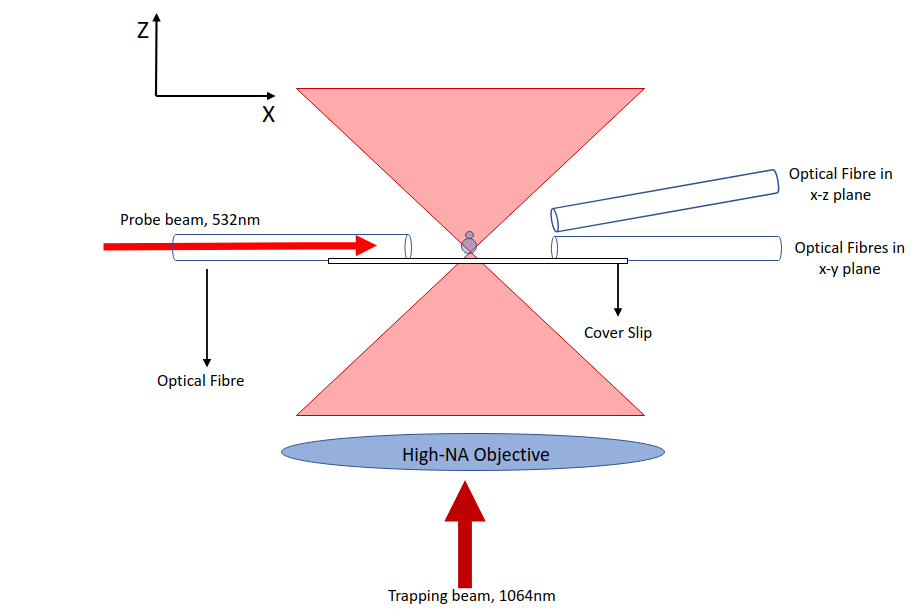
\includegraphics[width=\textwidth, height=0.25\textheight]{./Images/fig1a.png}
	\subcaption{}
\end{subfigure}
\begin{subfigure}{0.45\textwidth}
	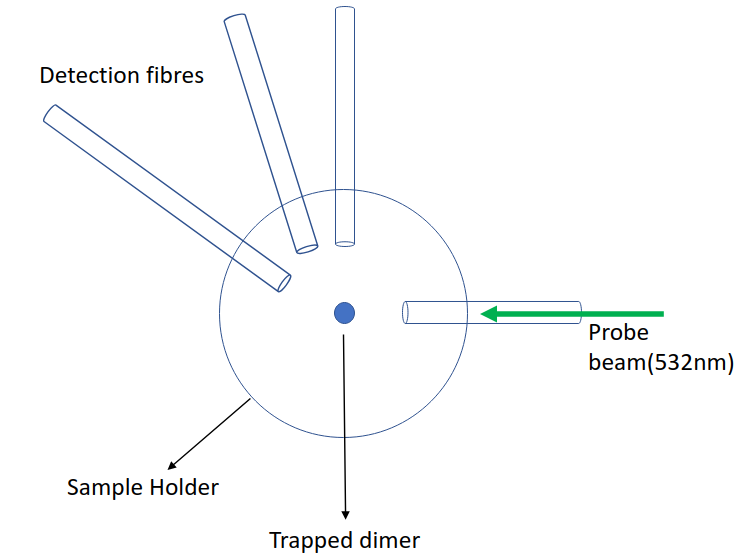
\includegraphics[width=\textwidth, height=0.25\textheight]{./Images/fig1b.png}
	\subcaption{}
\end{subfigure}
\caption{\label{fig:setup}
  %
  Experimental set up, a) Side view, b) Top view
%
}
\end{figure}


%%%%%%%%%%%%%%%%%%%%%%%%%%%%%%%%%%%%%%%%%%%%%%%%%%%%%%%%%%%%%%%%%%%%%%%%%%%%%%%%
%%%%%%%%%%%%%%%%%%%%%%%%%%%%%%%%%%%%%%%%%%%%%%%%%%%%%%%%%%%%%%%%%%%%%%%%%%%%%%%%
\section{Methodology}
\label{sec:Method}

\subsection{Brownian Simulation}
\label{sec:2.1}

We use the Brownian OT package developed by Fung~\textit{et~al}.
\cite{Vigilante2020Brownian_OT} to simulate the motion of a asymmetric
dimer within an optical trap.  Brownian OT combines MSTM
\cite{Mishchenko1996MSTM} and ``Optical Tweezer Toolbox''
(\textit{ott}) \cite{Lenton2020} to simulate the motion of arbitrary
shaped sphere clusters.  We simulated the motion of silica dimer
trapped in a $5$\,mW Gaussian beam; the dimer was comprised of two
spheres with radii $1\,{\rm \mu m}$ and $ 0.5\,{\rm \mu m}$,
respectively.  We ran our simulation over the span of 10 seconds, with
Brownian OT calculating the dimer's orientation and position every
$1 \ ms$.


\begin{figure}[h]
	\centering
	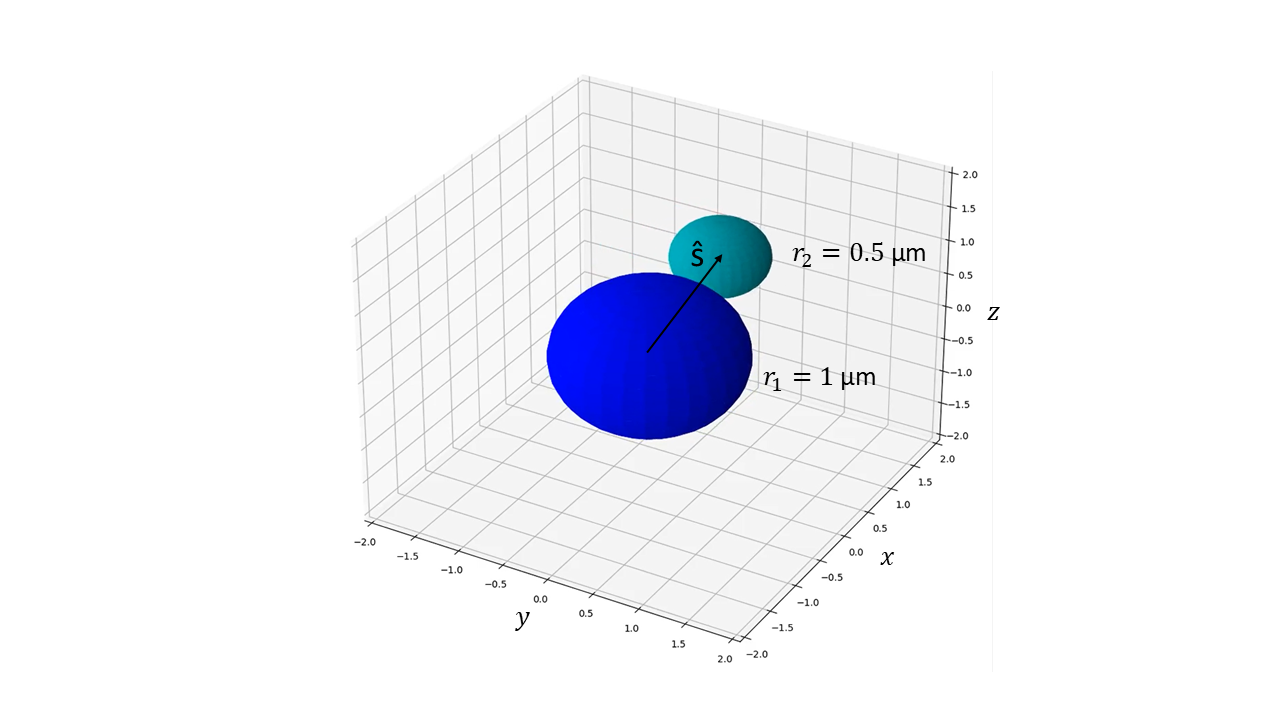
\includegraphics[width=0.9\textwidth]{./Images/Dimer.png}
	\caption{Example dimer in orientation $\bar{\bf s}$}
	\label{fig:dimer}
\end{figure}

With any trapped particle there are two main sources of motion,
Brownian and optical forces.  The dimer's Brownian motion
($\Delta q^{\textbf{B}}$) is simulated by generating a set of
normally-distributed numbers whose covariance is given by the dimer's
diffusion tensor $\textbf{D}$.  The diffusion tensor is computed based
on Farsund's work \cite{Farsund1996}. For computing the optical force
Brownian OT uses the T-Matrix method to calculate the scattering
coefficients of the outgoing scattered wave.  The T-matrix describes
the scattering process by relating the scattering wave to the incident
wave:
\begin{align}
	\begin{pmatrix}
		p_{mn} \\
		q_{mn}
	\end{pmatrix}
	= \textbf{T}
	\begin{pmatrix}
		a_{mn} \\
		b_{mn}
	\end{pmatrix}
\end{align}
MSTM computes the T-matrix of the dimer, and then passes the T-matrix
to \textit{ott} to compute the optical forces. The benefit of this
approach is that MSTM can accurately compute the T-matrix for any
arbitrary collection of spheres once, and then \textit{ott} can
calculate the optical forces and torques. The total displacement is
the sum of the optical and Brownian contributions:
\begin{align}
  \langle \Delta q_i^{\textbf{B}} \Delta q_j^{\textbf{B}}\rangle
  &= 2D_{ij} \Delta t
  \\
  \Delta q^{opt} &= \frac{\Delta t}{k_BT}\textbf{D} \cdot \textbf{F}
  \\
\Delta q^{tot} &= \Delta q^{\textbf{B}} + \Delta q^{opt}
\end{align}
where \textbf{F} is the a 6-component vector that describes the
optical force and torque components.  Brownian OT returns the dimer's
motion as a \textit{csv} file containing for each timestep the
$[x,y,z]$ position of the dimer's centre of mass relative to the trap
focus, and the orientation represented as a quaternion.


%%%%%%%%%%%%%%%%%%%%%%%%%%%%%%%%%%%%%%%%%%%%%%%%%%%%%%%%%%%%%%%%%%%%%%%%%%%%%%%%
\subsection{Orientation estimation from scattering measurements}
\label{sec:2.2}

We represent the instantaneous orientation of the moving dimer in the
trap as a unit vector $\hat{\bf s}$, pointing from the centre of the
larger sphere to the centre of the smaller sphere.  A plane wave
``probe'' laser beam directed perpendicular to the trapping laser,
incident on the dimer, generates a scattering pattern dependent on the
dimer's instantaneous orientation, $I(\bar{\bf s},\theta_k)$.  This
scattering pattern was computed using MSTM for each time step of the
Brownian dynamics simulation.  To represent a simulated measurement,
three angles ($\theta_1$, $\theta_2$, $\theta_3$) were chosen, and the
calculated intensity at each angle $\theta_k$ is recorded as
$I(\hat{\bf s}, \theta_k)$.

Our goal is to estimate the dimer orientation $\bar{\bf s}$ over time,
based on the scattering measurements $I(\bar{\bf s},\ \theta_k)$: the
question then is what set of angles ($\theta_1$, $\theta_2$,
$\theta_3$) give us the most useful information on $\hat{\bf s}$.  To
initially simplify the problem, rather than trying to get an exact
estimation of $\hat{\bf s}$, we discretise the orientation into
$n_{\rm ref}=30$ possible reference orientations $\hat{\bf n}_\alpha$
that are evenly distributed on the unit sphere \cite{Rey2006}.
%
We then consider how to optimise an experiment to identify the
reference orientation $\hat{\bf n}_\alpha$ that is closest to the
actual orientation $\hat{\bf s}$ of the dimer.
%
The method can be extended to an arbitrarily large number of reference
orientations, but for clarity and practicability we use a relatively
small number here; additionally, the choice of a small number of
discrete reference or ``candidate'' orientations also accounts for the
fact that any experiment will necessarily have a limited precision.
%
Using MSTM we compute the scattering that would be produced by the
dimer in each of the reference orientations, denoted as
$I(\hat{\bf n}_\alpha, \theta)$ and obtain ``measurements''
$I(\hat{\bf n}_\alpha, \theta_k)$ at our chosen set of angles
($\theta_1$, $\theta_2$, $\theta_3$).
%
These raw intensities are normalised according to
\begin{align}
\label{eq:scale}
  y_k(\hat{\bf n}_\alpha)
  = 
  \frac{I(\hat{\bf n}_\alpha, \theta_k) - \langle I(\hat{\bf n},\theta_k) \rangle } 
  {\langle I^2(\hat{\bf n},\theta_k) \rangle -\langle I(\hat{\bf n}, \theta_k)\rangle^2}
\end{align}
where the denominator is simply the standard deviation for our values
of $I(\hat{\bf n}, \theta_k)$.  The dimer's \emph{actual}
instantaneous scattered intensity, based on the real instantaneous
orientation $\bar{\bf s}$, is similarly scaled using
Eq.~\eqref{eq:scale} to give $y(\bar{\bf s},\theta_k)$.
%
The reference orientations, raw intensities, and scaled signals are
given in Tables~\ref{tab:A1} and \ref{tab:A2}.
%
In practice, $y_k(\bar{\bf s})$ will have an inherent amount of
uncertainty in our measurement due to noise from our detector.  We
compare our instantaneous signal to our reference signal by assuming
that the measurement uncertainty for each detection fibre is Gaussian
and is centred about $y_k(\bar{\bf s})$ Combining all three detection
angles provides us with the conditional probability that, should the
dimer be in orientation $\hat{\bf n}_\alpha$, it would produce a
signal $y(\bar{\bf s})$:
\begin{align}
\label{eq:conditional}
  p(y(\bar{\bf s})|\hat{\bf n}_\alpha)
  = \prod^3_{k=1}
(2\pi\sigma_k^2)^{-1/2} 
e^{-(y_{k}(\hat{\bf n}_\alpha)-y_{k}(\bar{\bf s}))^2/2\sigma_k^2}
\end{align}
where $\sigma_k$ is related to the uncertainty in the detected signal
from our dimer $y_k(\bar{\bf s})$.  We left this as a tuneable
parameter to characterize the influence of experimental error on our
predictive method.  The signal error was simulated in our model by
stochastically adjusting our values of $y_k(\bar{\bf s})$.
\begin{eqnarray*}
  \sigma_k
  &= \epsilon\bar{y}(\hat{\bf n}_k)
  \\
  \Rightarrow y(\bar{\bf s}_k) &= y(\bar{\bf s})_k \pm n\sigma_k
  \\ 
n \in \mathbb{R}, n\in[0,1]
\end{eqnarray*} 
where $\epsilon$ is the percent error expected from our detection
fibres.  Equation~\eqref{eq:conditional} assigns a probability to each
reference orientation based on how similar the ``reference orientation
signal'' $y_{k}(\hat{\bf n}_\alpha)$ is to the actual signal
$y_{k}(\bar{\bf s})$ generated by the dimer in its real orientation
$\bar{\bf s}$.  However, if our values of $y_k(\hat{\bf n}_\alpha)$
are similar to one another, the probability distribution from
Eq.~\eqref{eq:conditional} will therefore assign similar probability
for multiple reference orientations. Bayesian inference allows one to
update a probability distribution by accounting for information known
prior to making a measurement.  We apply this by accounting for our
distribution of reference orientations and instantaneous signals.
\begin{align}
  \label{eq:bayes}
  p(\hat{\bf n}_\alpha| y_1,y_2,y_3)
  &=
    \frac{p(y_1,y_2,y_3|\hat{\bf n}_\alpha)
    p(\hat{\bf n}_\alpha)}{p(y_1, y_2, y_3)}
\end{align}
where $p(\hat{\bf n}_\alpha)$ and $p(y_1, y_2, y_3)$ are the prior
estimates of the distributions of particle orientations and
instantaneous signals, respectively.  The former can be estimated by
some Boltzmann distribution based on how far apart reference
orientations are in physical space, covered in Section~\ref{sec:2.3}.
The latter prior $p(y)$ is the probability of our dimer producing a
signal $y_k(\bar{\bf s})$ that falls with our distribution of
reference signals $y_k(\hat{\bf n})$.  This is given by taking the
discrete integral over collection of reference orientations.
\begin{align}
  p(y_1, y_2, y_3)
  =
  \sum_{\alpha=1}^{n_{\rm ref}}
  p(y_1, y_2, y_3|\hat{\bf n}_\alpha)
  p(\hat{\bf n}_\alpha)
\end{align}
The implementation of Eq.~\eqref{eq:bayes} improves our estimate by
suppressing reference orientations that are far away from our dimer's
orientation vector in physical space.  In order to evaluate the
accuracy of our method, we tested it using a Brownian dynamics
simulation of the dimer (see Section~\ref{sec:2.1}).


%%%%%%%%%%%%%%%%%%%%%%%%%%%%%%%%%%%%%%%%%%%%%%%%%%%%%%%%%%%%%%%%%%%%%%%%%%%%%%%%
\subsection{Testing the Model}
\label{sec:2.3}


Using our simulation from Section~\ref{sec:2.1} we calculated the
instantaneous signal from our dimer at each time step using MSTM.  We
applied Eq.~\eqref{eq:bayes} --- covered in Section~\ref{sec:2.2} ---
and the reference orientation with the highest probability is taken as
our estimation of the dimer's instantaneous orientation.  The prior of
the reference orientations $p_i(\hat{\bf n})$ is defined at each time
step by accounting for the physical distance between our previous
estimation $\hat{\bf n}_{i, \ t - \Delta t}$ and each reference
orientation $\hat{\bf n}$
\begin{align}
  r_i(t, \hat{\bf n}_i)
  &= \frac{1}{2}((\hat{\bf n}_{i,\ t} \cdot \hat{\bf n}_{t-\Delta t})-1)
  \\
  p_i(\hat{\bf n})
  &= \frac{e^{\beta (r_i(t,\hat{\bf n}_i)-1)}}
{\sum_{j=1}^{30}e^{\beta(r_j(t, \hat{\bf n}_i)-1)}}
\end{align}
where $\beta$ is a weighting factor that controls the significance of
our priori estimate.  The simulation data from Section~\ref{sec:2.1}
was used to check if the estimation was correct by comparing the
estimate provided by Eq.~\eqref{eq:bayes} to the reference orientation
closest to the instantaneous orientation, denoted as
$\hat{\bf n}_{best}$.  To measure the error in the model's estimate
the distribution's of $p(\hat{\bf n}| y(\bar{\bf s}))$ and an
ideal result, $p_ideal$, were compared.  An ideal distribution is one
that is 0 for every $\hat{\bf n}$ apart from the correct result.
\begin{align}
p_{ideal} = 
\begin{cases}
	1 & \text{when $\hat{\bf n}_i$ = $\hat{\bf n}_{best}$}\\
	0 & \text{anywhere else}
\end{cases}
\end{align}
The distribution from Eq.~\eqref{eq:bayes} will assign some non-zero
probability to every reference orientation.  The model's error was
measured by calculating the Kullback-Leibler divergence $K_l$ between
the two distributions
\begin{align}
  K_{l, \#}(p_i(\hat{\bf n}| y_k(\bar{\bf s})) &\parallel p_{ideal}) =\nonumber
  \\
&p_{ideal}\ln \left[\frac{p_{ideal}}{p(\hat{\bf n}_{best}| y(\bar{\bf s}))}
\right]
\end{align}
where a more negative value of $K_l$ indicates a poorer estimation of
the dimer's instantaneous orientation.  By summing the divergence of
each measurement across the entire simulation we get an evaluation of
how well the model performed in estimating the dimer's orientation.
To compare between different iterations of our model the we compare
our result of $K_l$ to a worst case scenario and evaluate how much it
improves upon this, denoted as $F(K_l)$:
\begin{align}
K_{l, \ total} &= \sum\limits_{\# =1}^{timesteps} K_{l,\#} \\
K_{l, \ worst} &= -\sum\limits_{\#=1}^{timesteps} \ln \left[\frac{1}{1/30} \right] \\
F(K_l) &= \frac{K_{l,\ worst}}{K_{l, \ total}}
\end{align}

The worst case scenario is akin to randomly choosing a reference
orientation at each time step. The greater the value of $F(K_l)$ the
lower the error between our estimated orientation and the dimer's
instantaneous orientation. Because our model is dependent on several
parameters we need to a sophisticated method for understanding how
these parameters correlate with $F(K_l)$.


%%%%%%%%%%%%%%%%%%%%%%%%%%%%%%%%%%%%%%%%%%%%%%%%%%%%%%%%%%%%%%%%%%%%%%%%%%%%%%%%
\subsection{Optimization of parameters}
\label{sec:2.4}

The signal error $\epsilon$ and the weighting factor $\beta$ are known
quantities whose influence can be measured directly; however, our
choice of angles and how they correlate with $F(K_l)$ is not easily
understood Evaluating every possible configuration manually is
inefficient, therefore we utilised Ultra-nest to apply a Monte Carlo
simulation to our model. Ultra-nest is a sophisticated python package
for fitting models with complex parameter correlations
\cite{Buchner2016Ultranest}.  UltraNest implements a variation of
Monte Carlo integration, nested-sampling, where a likelihood contour
is used to update a group of live points chosen from the prior
estimation ($0^{\circ} \leq \theta_k \leq 180^{\circ}$).

The UltraNest software was used to create a set of live points of
different choices of $\theta_1$, $\theta_2$, and $\theta_3$, with each
point being evaluated by its improvement factor ($F(K_l)$).  After
evaluating every live point, the worst results are removed and new
live points are created based on the information provided by the
previous live points.  If there is a correlation between the choice of
angles and $F(K_l)$ then the live points should congregate around a
single (or multiple) choice of angles that will maximise $F(K_l)$ and
therefore minimise the error between our estimate and instantaneous
orientation.


%%%%%%%%%%%%%%%%%%%%%%%%%%%%%%%%%%%%%%%%%%%%%%%%%%%%%%%%%%%%%%%%%%%%%%%%%%%%%%%%
%%%%%%%%%%%%%%%%%%%%%%%%%%%%%%%%%%%%%%%%%%%%%%%%%%%%%%%%%%%%%%%%%%%%%%%%%%%%%%%%
\section{Results and  Discussion}
\label{sec:Discussion}


%%%%%%%%%%%%%%%%%%%%%%%%%%%%%%%%%%%%%%%%%%%%%%%%%%%%%%%%%%%%%%%%%%%%%%%%%%%%%%%%
\subsection{Asymmetric dimer dynamics}
\label{sec:3.1}

The Brownian OT software was used to simulate the motion of a trapped
dimer ($a_1=1\mu m, a_2=0.5\mu m$) over the first $10$\,seconds of
entering the optical trap.  The initial orientation was assumed as
strictly vertical (in line with the beam propagation direction). The
dimer's position orientation was recorded every $10\,{\rm \mu s}$ for
using as a test dataset for our model.

\begin{figure}[h]
	\label{fig:motion}
	\centering
	\begin{subfigure}{0.45\textwidth}
		\subcaption{}
		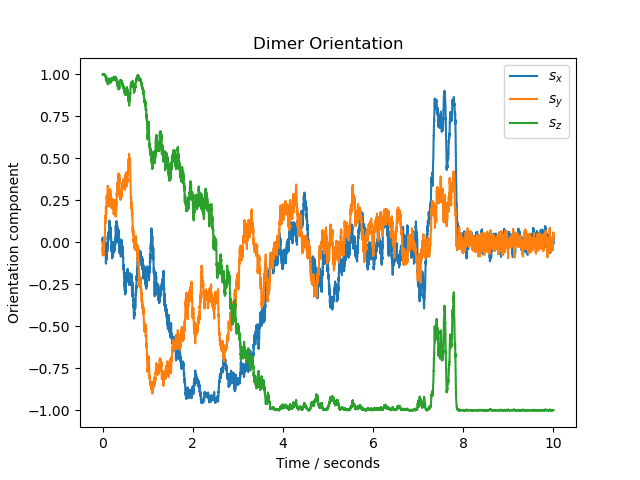
\includegraphics[width =\textwidth]{./Images/traj.png}
	\end{subfigure}
	\begin{subfigure}{0.45\textwidth}
		\subcaption{}
		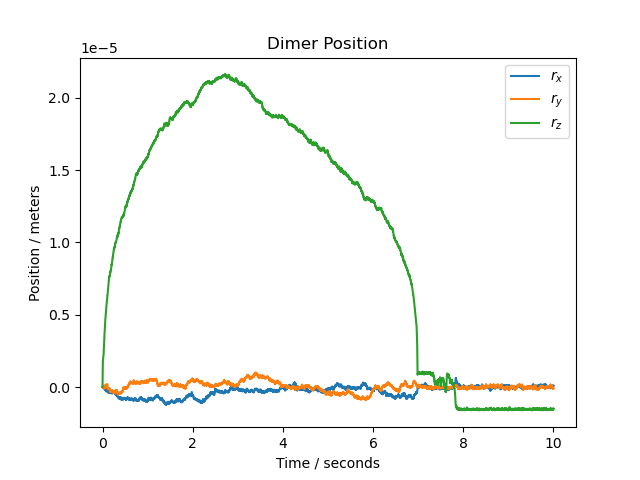
\includegraphics[width=\textwidth]{./Images/pos.png}
	\end{subfigure}
	\caption{Simulation results of: a) the dimers orientation vector with time, b) the dimer's [x,y,z] position with time.}
\end{figure}

As can be seen from Figure~\ref{fig:motion}, the dimer undergoes a
full $180^{\circ}$ rotation upon entering the trap. Typically
horizontal alignment of a dimer is unstable and will result in the
particle rotating to align along its vertical axis. It is interesting
to note that the dimer is furthest from the trap centre as it goes
into a horizontal orientation before drawing closer again as it
inverts completely. Further simulations of differently sized dimers
showed similar results, but only when $a_1 \geq 2a_2$. Dimers with
more symmetrical size ratios immediately aligned into a fixed vertical
position.
%
In Vigilante's work with dimers \cite{Vigilante2020Brownian_OT}
simulations of trapped symmetrical dimers was investigated; their
findings showed that the optical torque on the dimer goes to zero
while aligned vertically and is at its maximum in a horizontal
alignment.  Therefore, the inversion of an asymmetric dimer suggests
that if the size difference is significant the optical torque goes is
minimal for a dimer in both horizontal and vertical orientations. Once
we have our experimental set up complete we can confirm this by
trapping an asymmetric dimer and monitoring its orientation. The data
from \figurename{ 2a} was used to test the efficacy of our predictive
model. To visualise how well our model tracks the dimer's orientation
we plot the radial distance between our model's prediction and the
true orientation, and between the best possible orientation and the
true orientation. For a perfect estimation these two plots should
overlap, while we cannot achieve an exact estimation we can optimise
it by adjusting the expected signal error and weighting factor.


%%%%%%%%%%%%%%%%%%%%%%%%%%%%%%%%%%%%%%%%%%%%%%%%%%%%%%%%%%%%%%%%%%%%%%%%%%%%%%%%
\subsection{Impact of signal error on model predictions}
\label{sec:3.2}

A key assumption of Eq.~\eqref{eq:conditional} is that we assume our
detected light signal will inherently have some degree of noise. This
is the central premise that allows us to form
Eq.~\eqref{eq:conditional}, understanding the limits of acceptable
signal error is necessary for implementing this to experimental work.
To this end we ran our model while varying the value of $\epsilon$.
\figurename{ 3} shows the performance of the method with a selection
of angles $15^{\circ}$, $55^{\circ}$, and $90^{\circ}$ and $\beta$ set
to $1$.  The dotted line indicates the minimum radian distance
($0.137$ radians) between two neighbouring reference orientations, if
we are under this line then we know our model is just off from
selecting the correct orientation


\begin{figure}[h]
	
	\centering
	\begin{subfigure}{0.49\textwidth}
		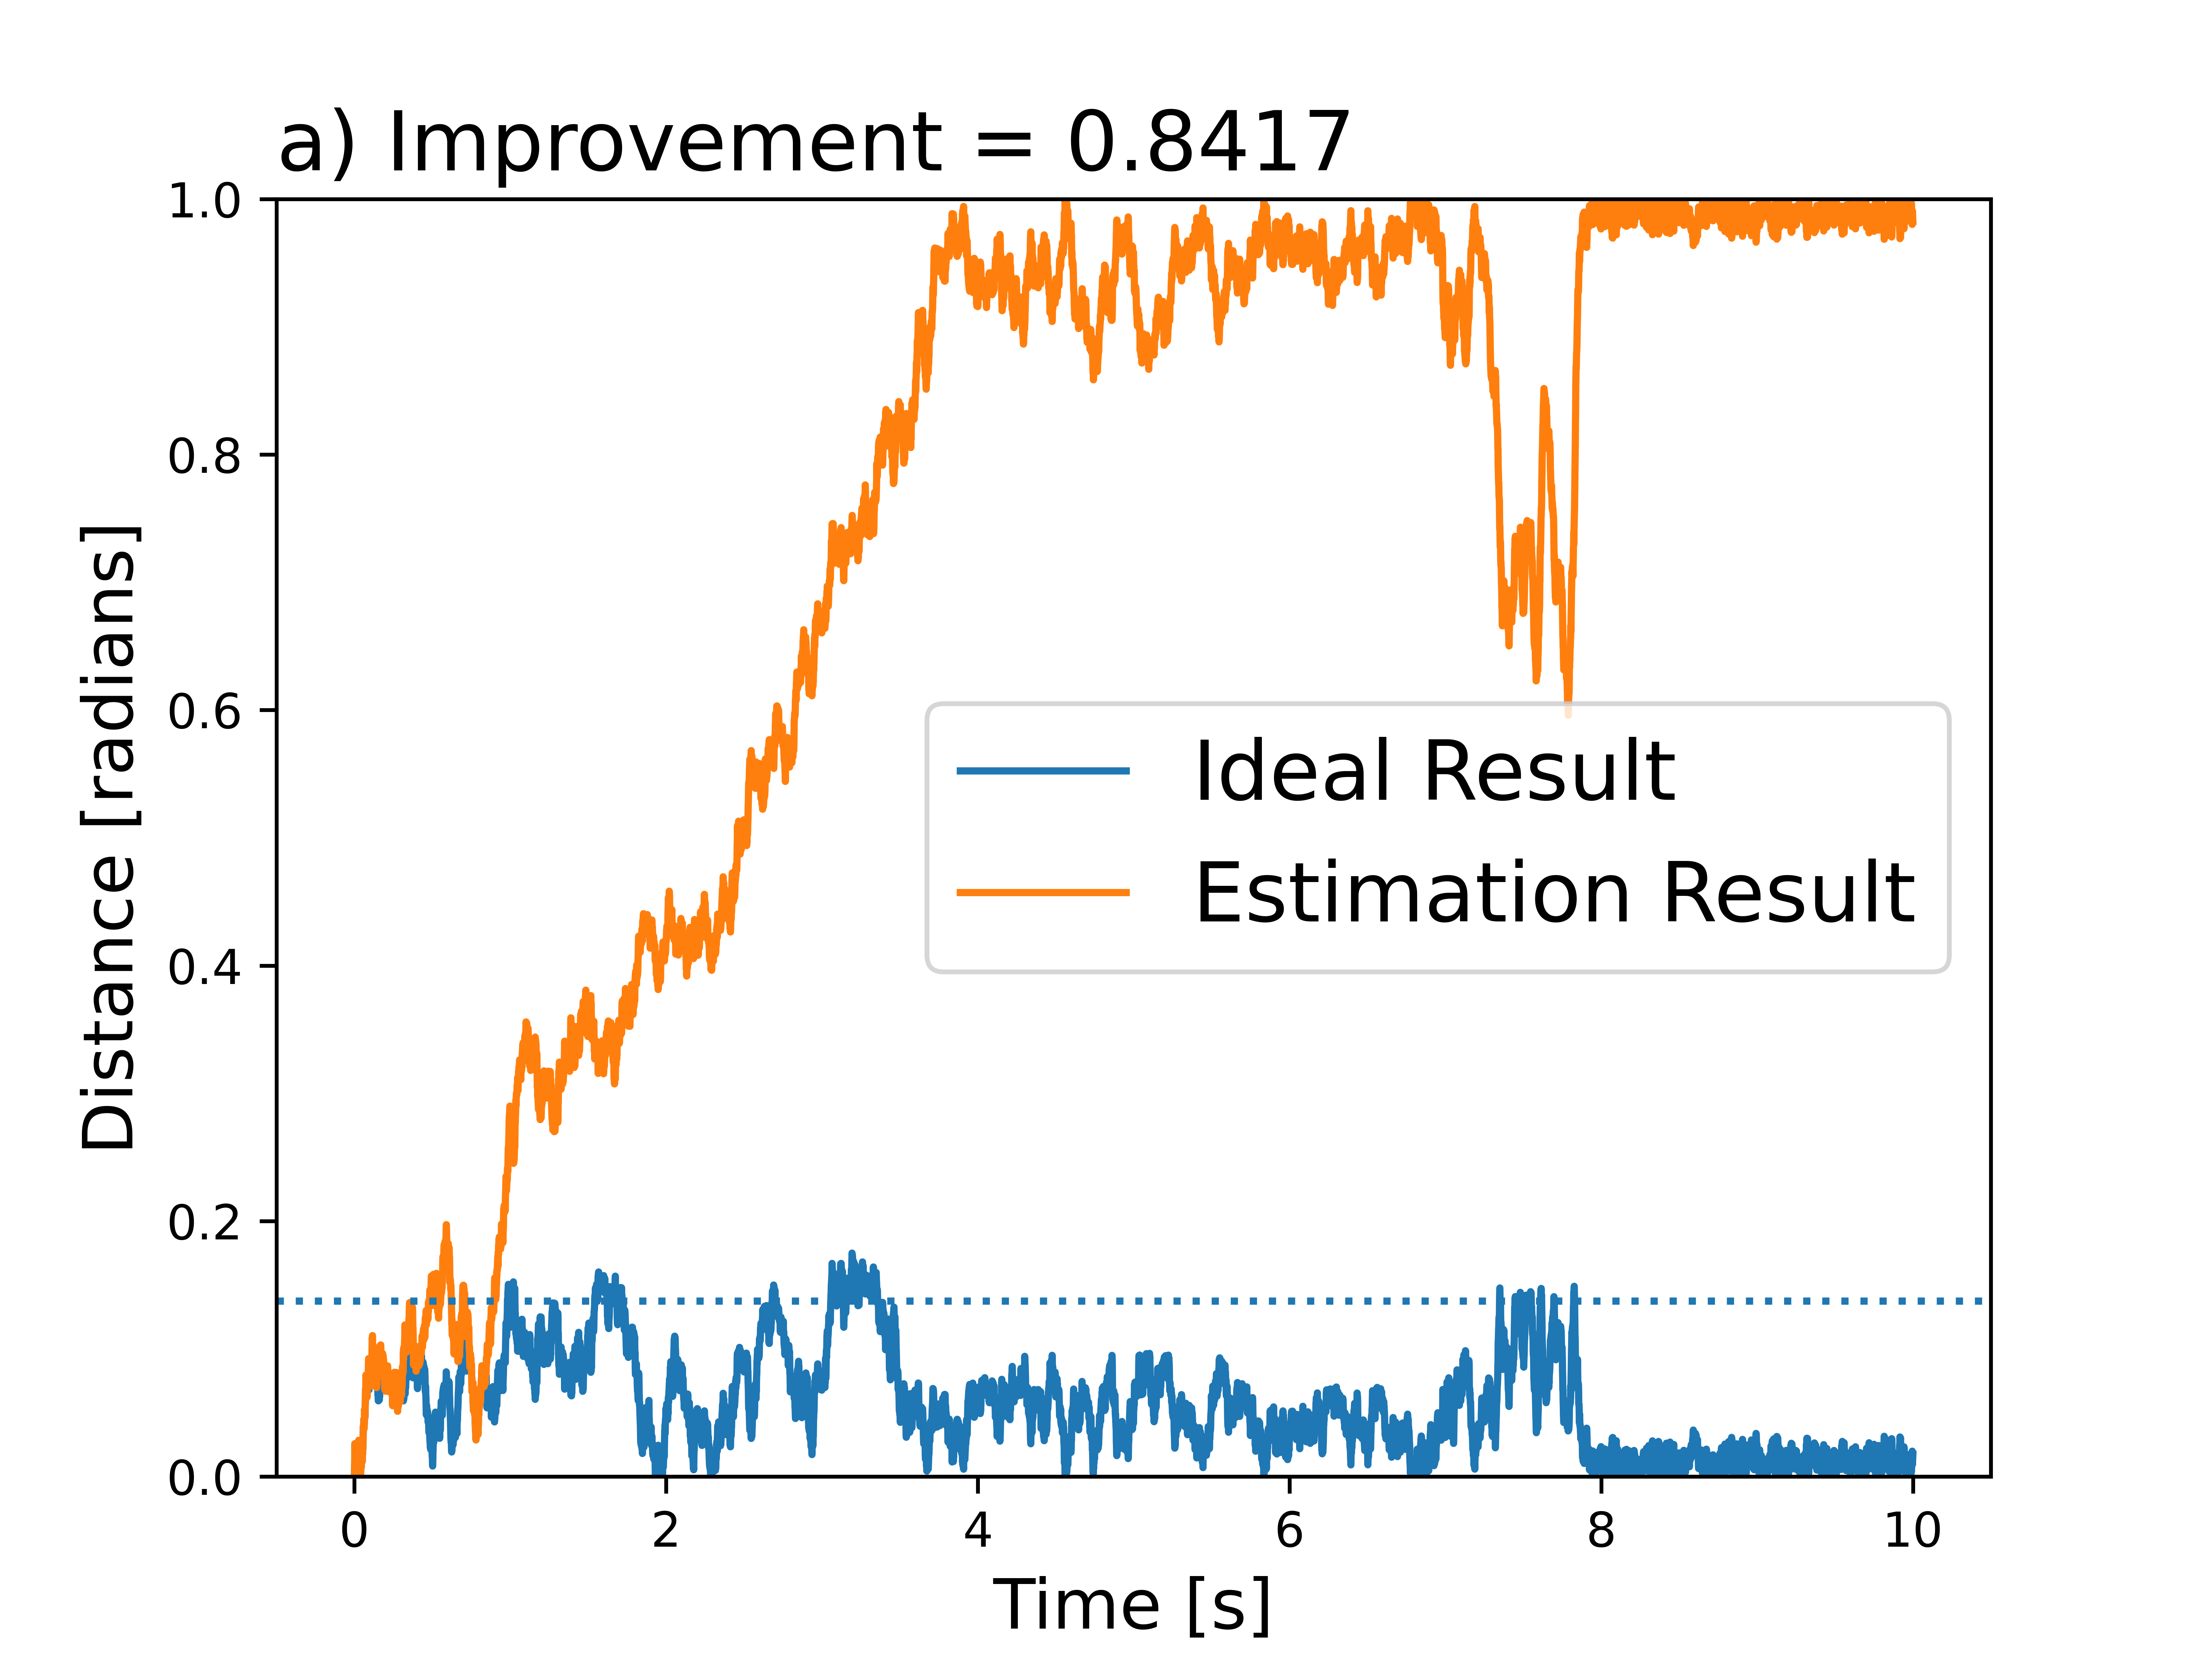
\includegraphics[width=\textwidth]{./Images/epsilon_5.png}
	\end{subfigure}
	\begin{subfigure}{0.49\textwidth}
		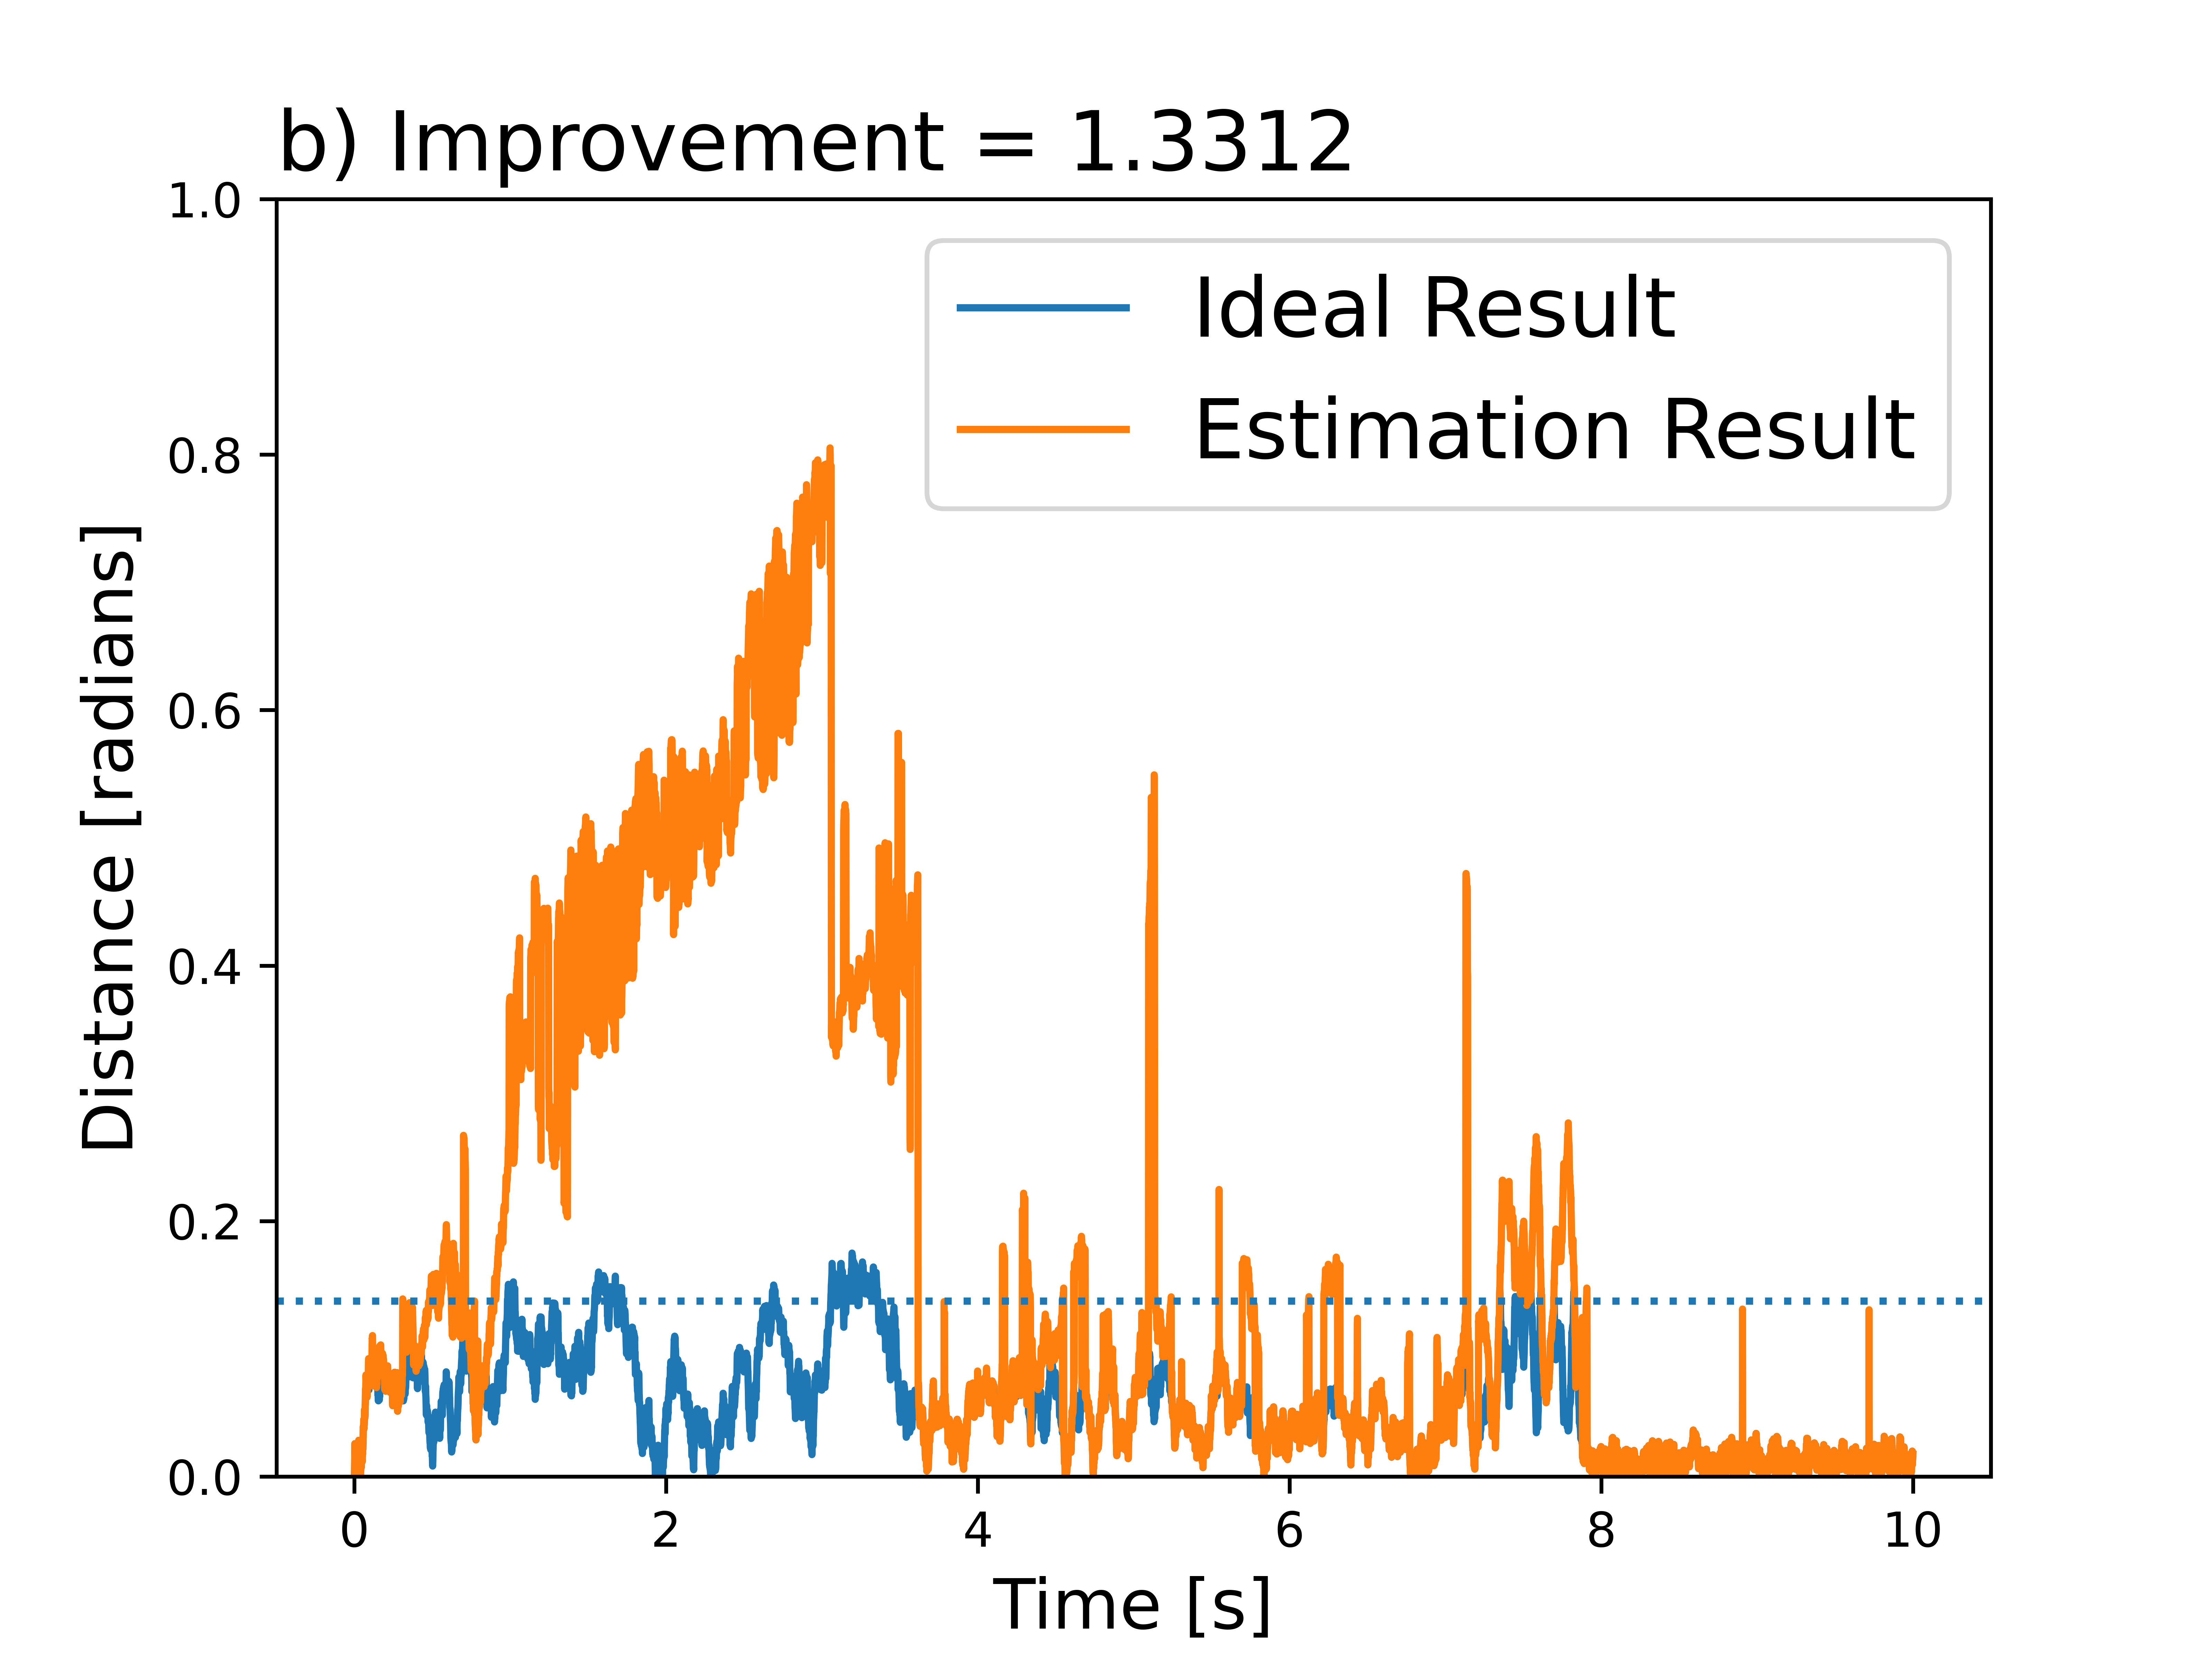
\includegraphics[width=\textwidth]{./Images/epsilon_15.png}
	\end{subfigure}
	\begin{subfigure}{0.5\textwidth}
		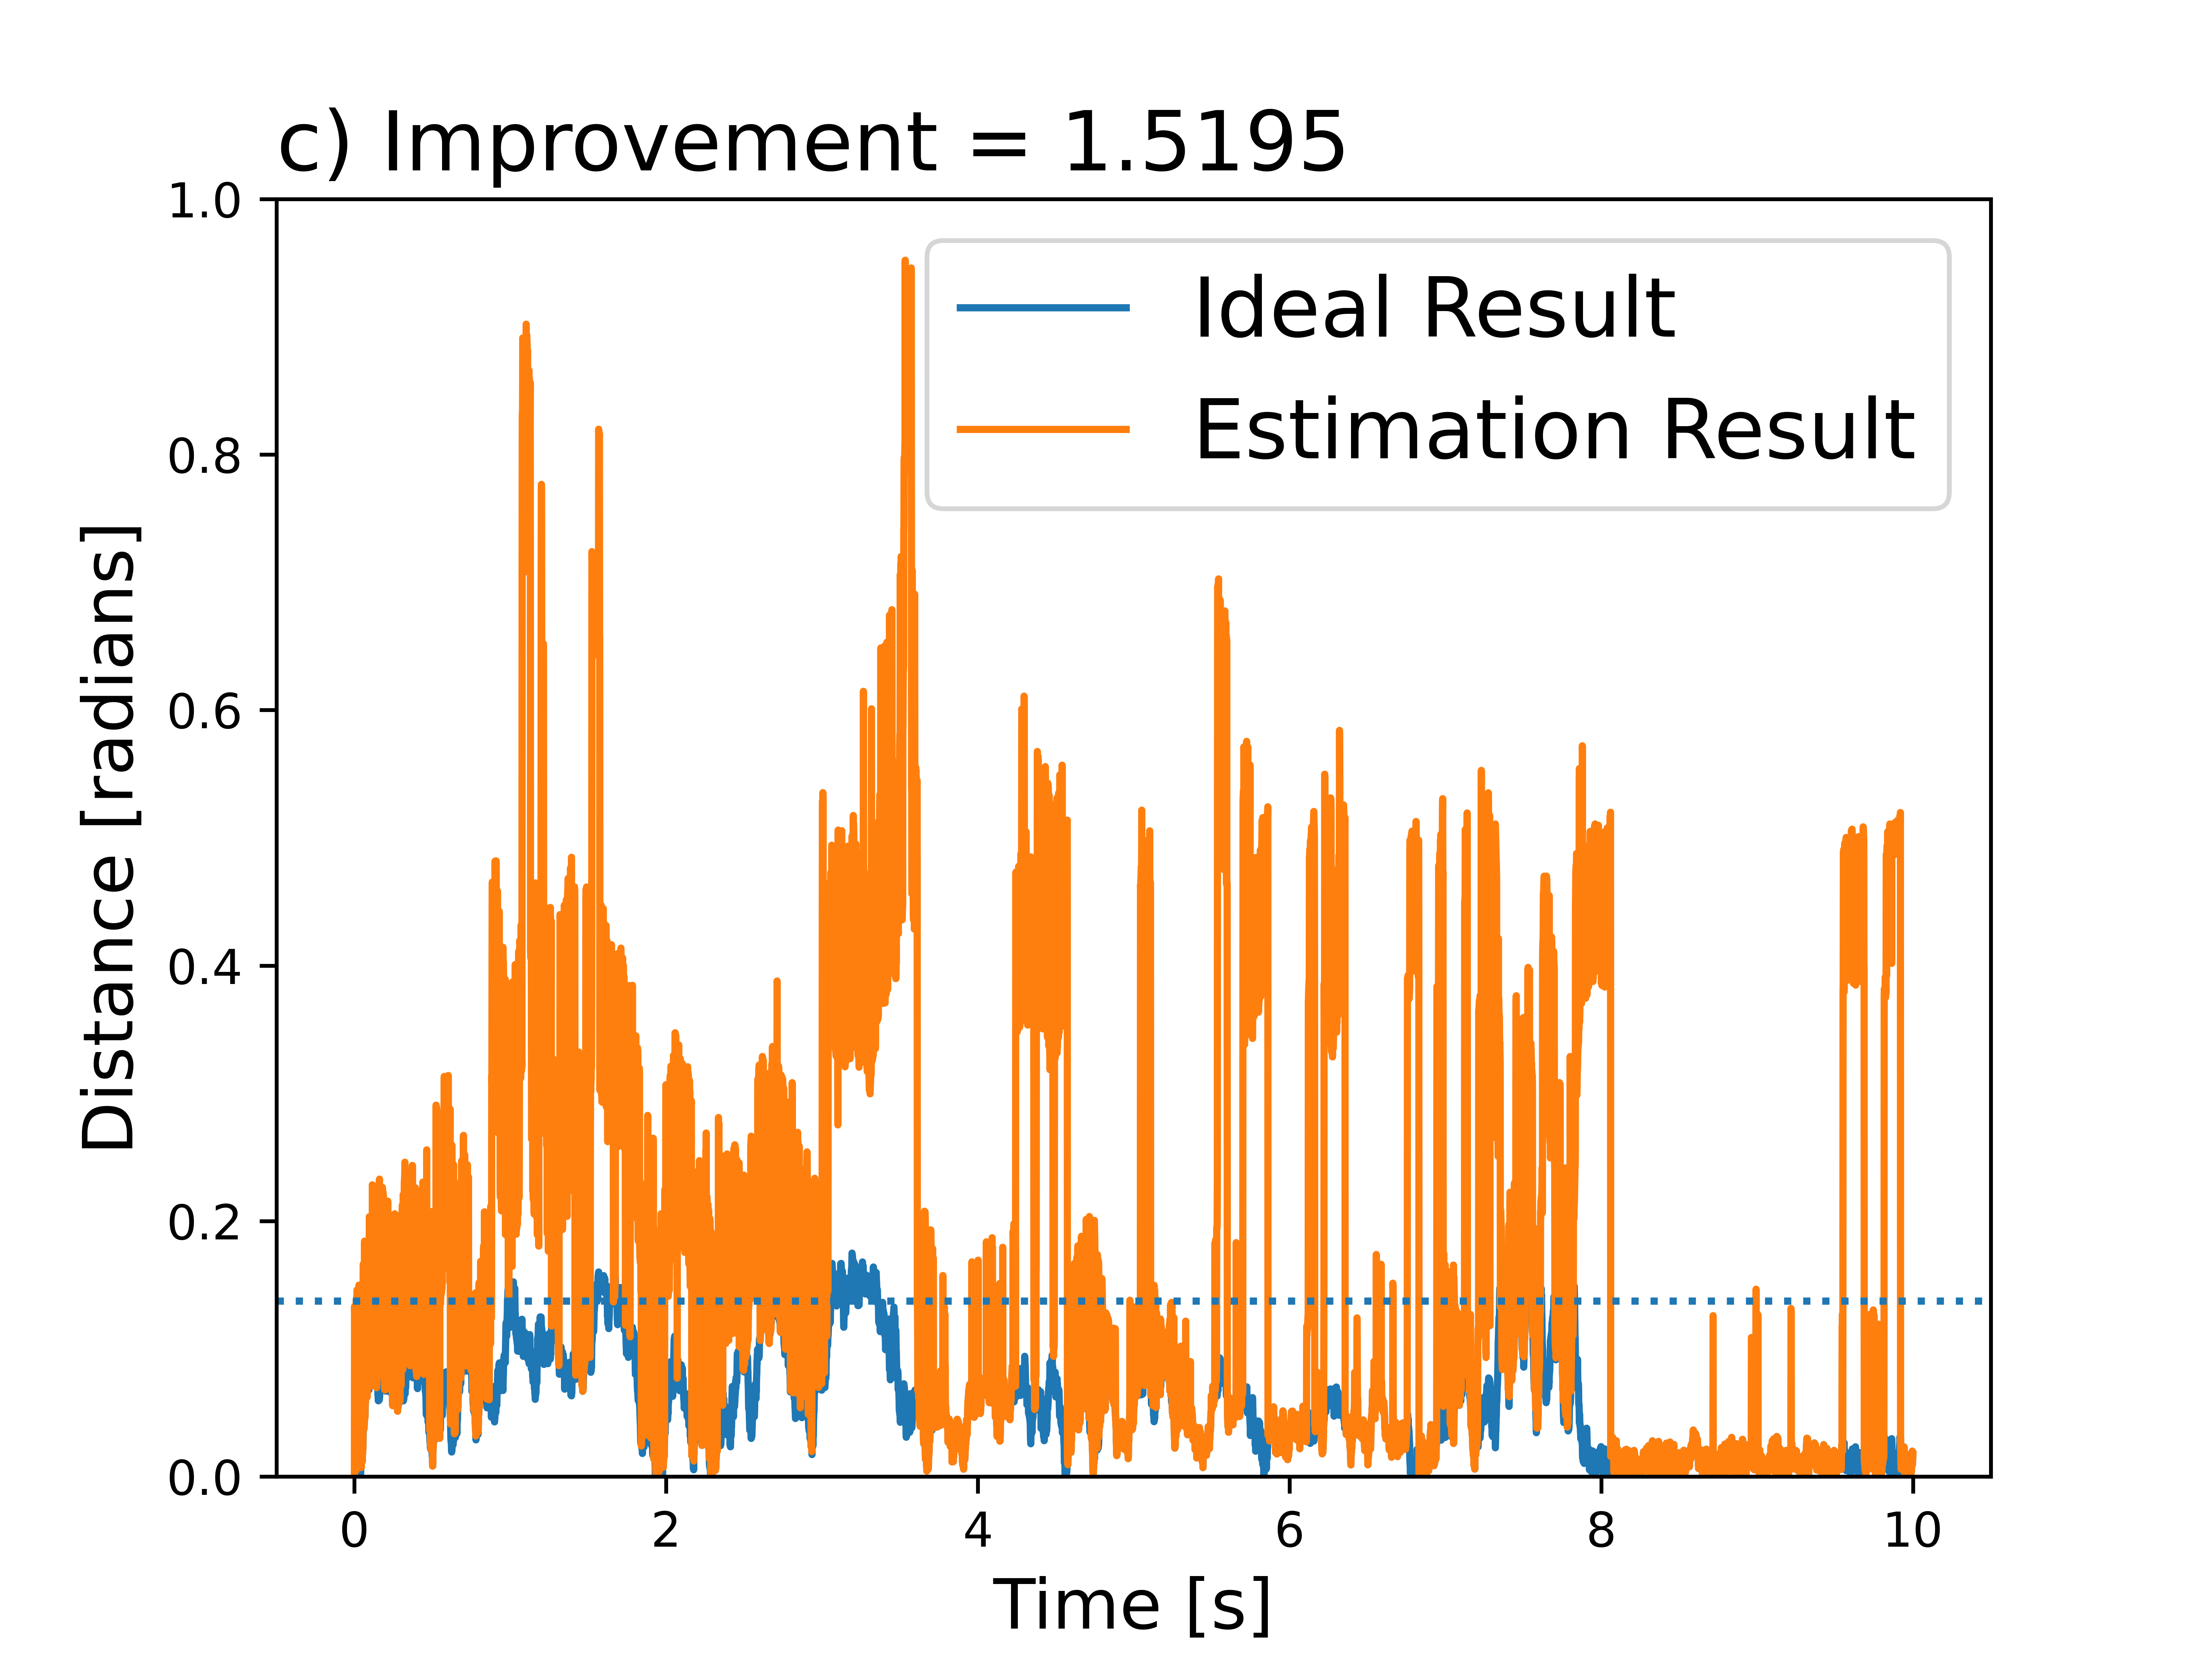
\includegraphics[width=\textwidth]{./Images/epsilon_25.png}
	\end{subfigure}
	\caption{Model prediction for signal error of a) $5\%$, b) $15\%$, and c) $25\%$. Blue line denotes the best result we can achieve, orange line denotes the result provided by eq~\ref{eq:bayes}}
	\label{fig:epsilon}
\end{figure}


As can be seen from Figure~\ref{fig:epsilon}, there is seemingly a
sweet spot for the signal error; with a $5$\% error giving an
inaccurate estimation, and with a $25$\% error giving an alright
estimation but with sudden shifts away from the ideal result. The
reason why our low error estimation performed so poorly is that the
minimum difference between our values of $y_k$ is larger than our
signal error.  As such the model could not distinguish between
different reference orientations and was essentially just picking
options at random.  This minimum difference determined by our choice of
angles and sets a lower limit of how accurate our signals can be.  In
the future we hope to look at increasing the number of reference
orientations to see what the true lower bound is.

The latter issue of a high signal error can be addressed somewhat by
adjusting our value of $\beta$ to flatten our probability
distribution. We repeated our model estimation at $25\%$ at different
values of $\beta$ to see the upper limit we could improve our result
to.

\begin{figure}
	\label{fig:beta}
	\centering
	\begin{subfigure}{0.49\textwidth}
		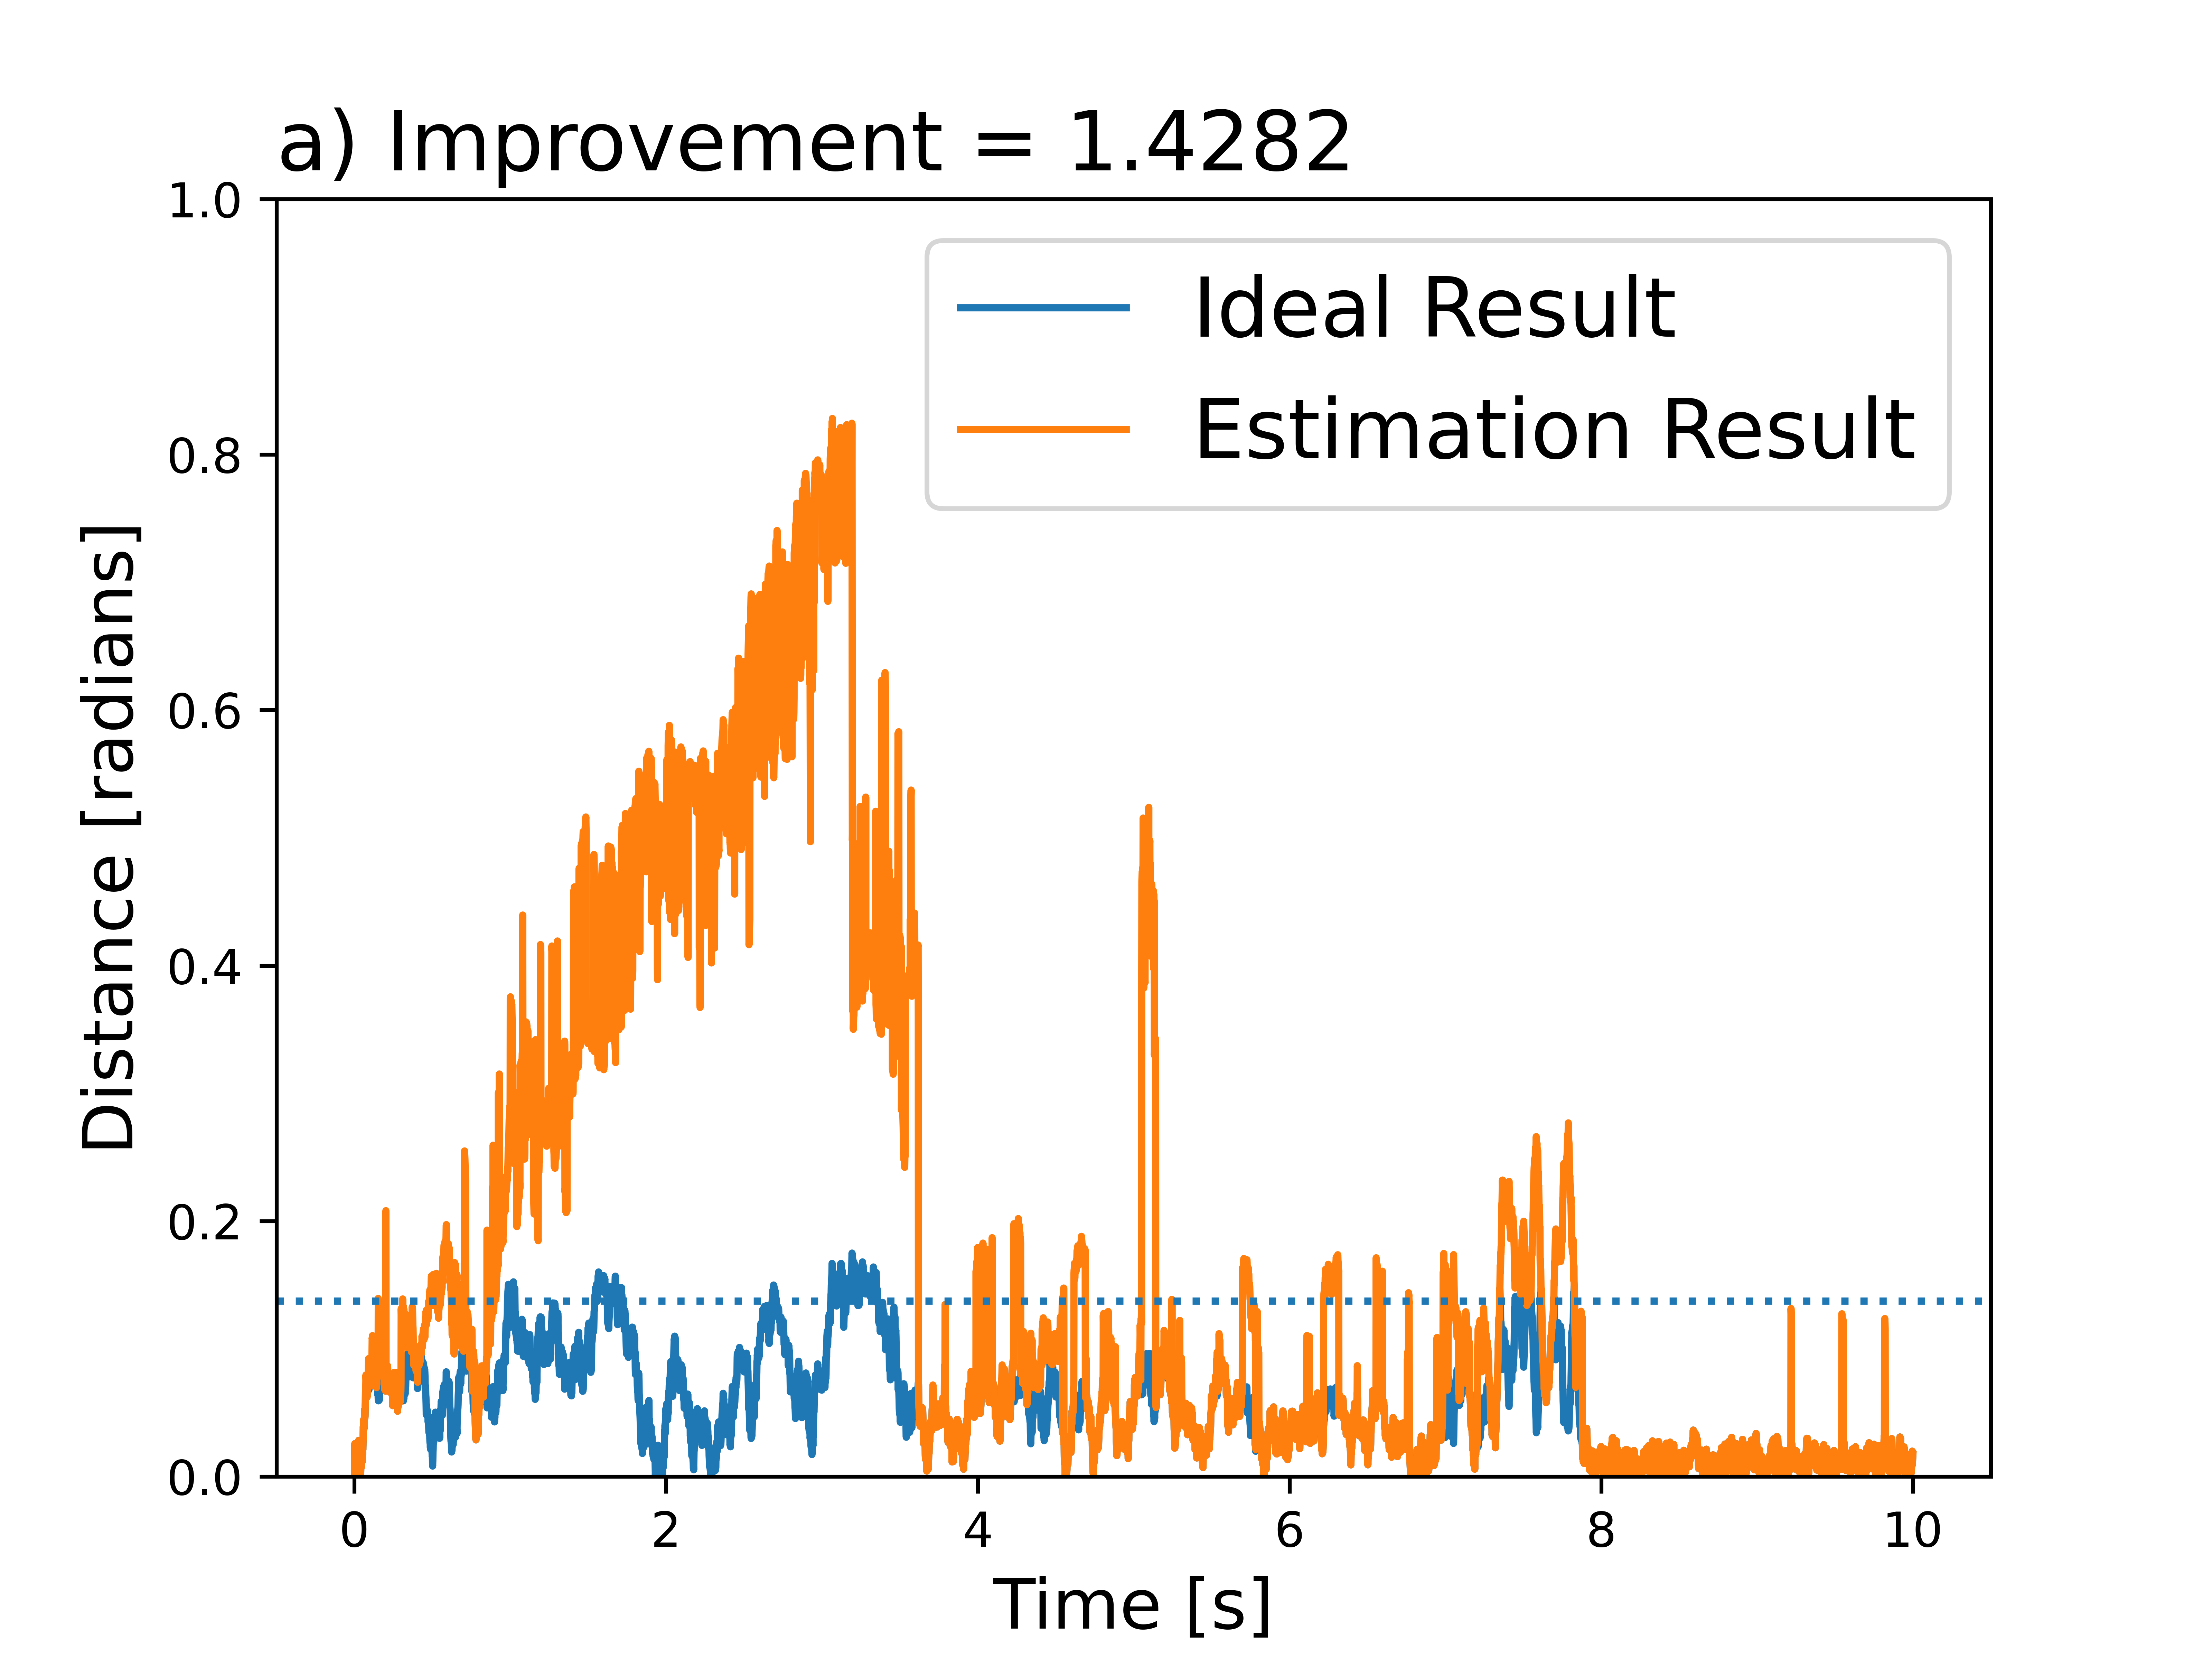
\includegraphics[width=\textwidth]{./Images/beta_5.png}
	\end{subfigure}
	\begin{subfigure}{0.49\textwidth}
		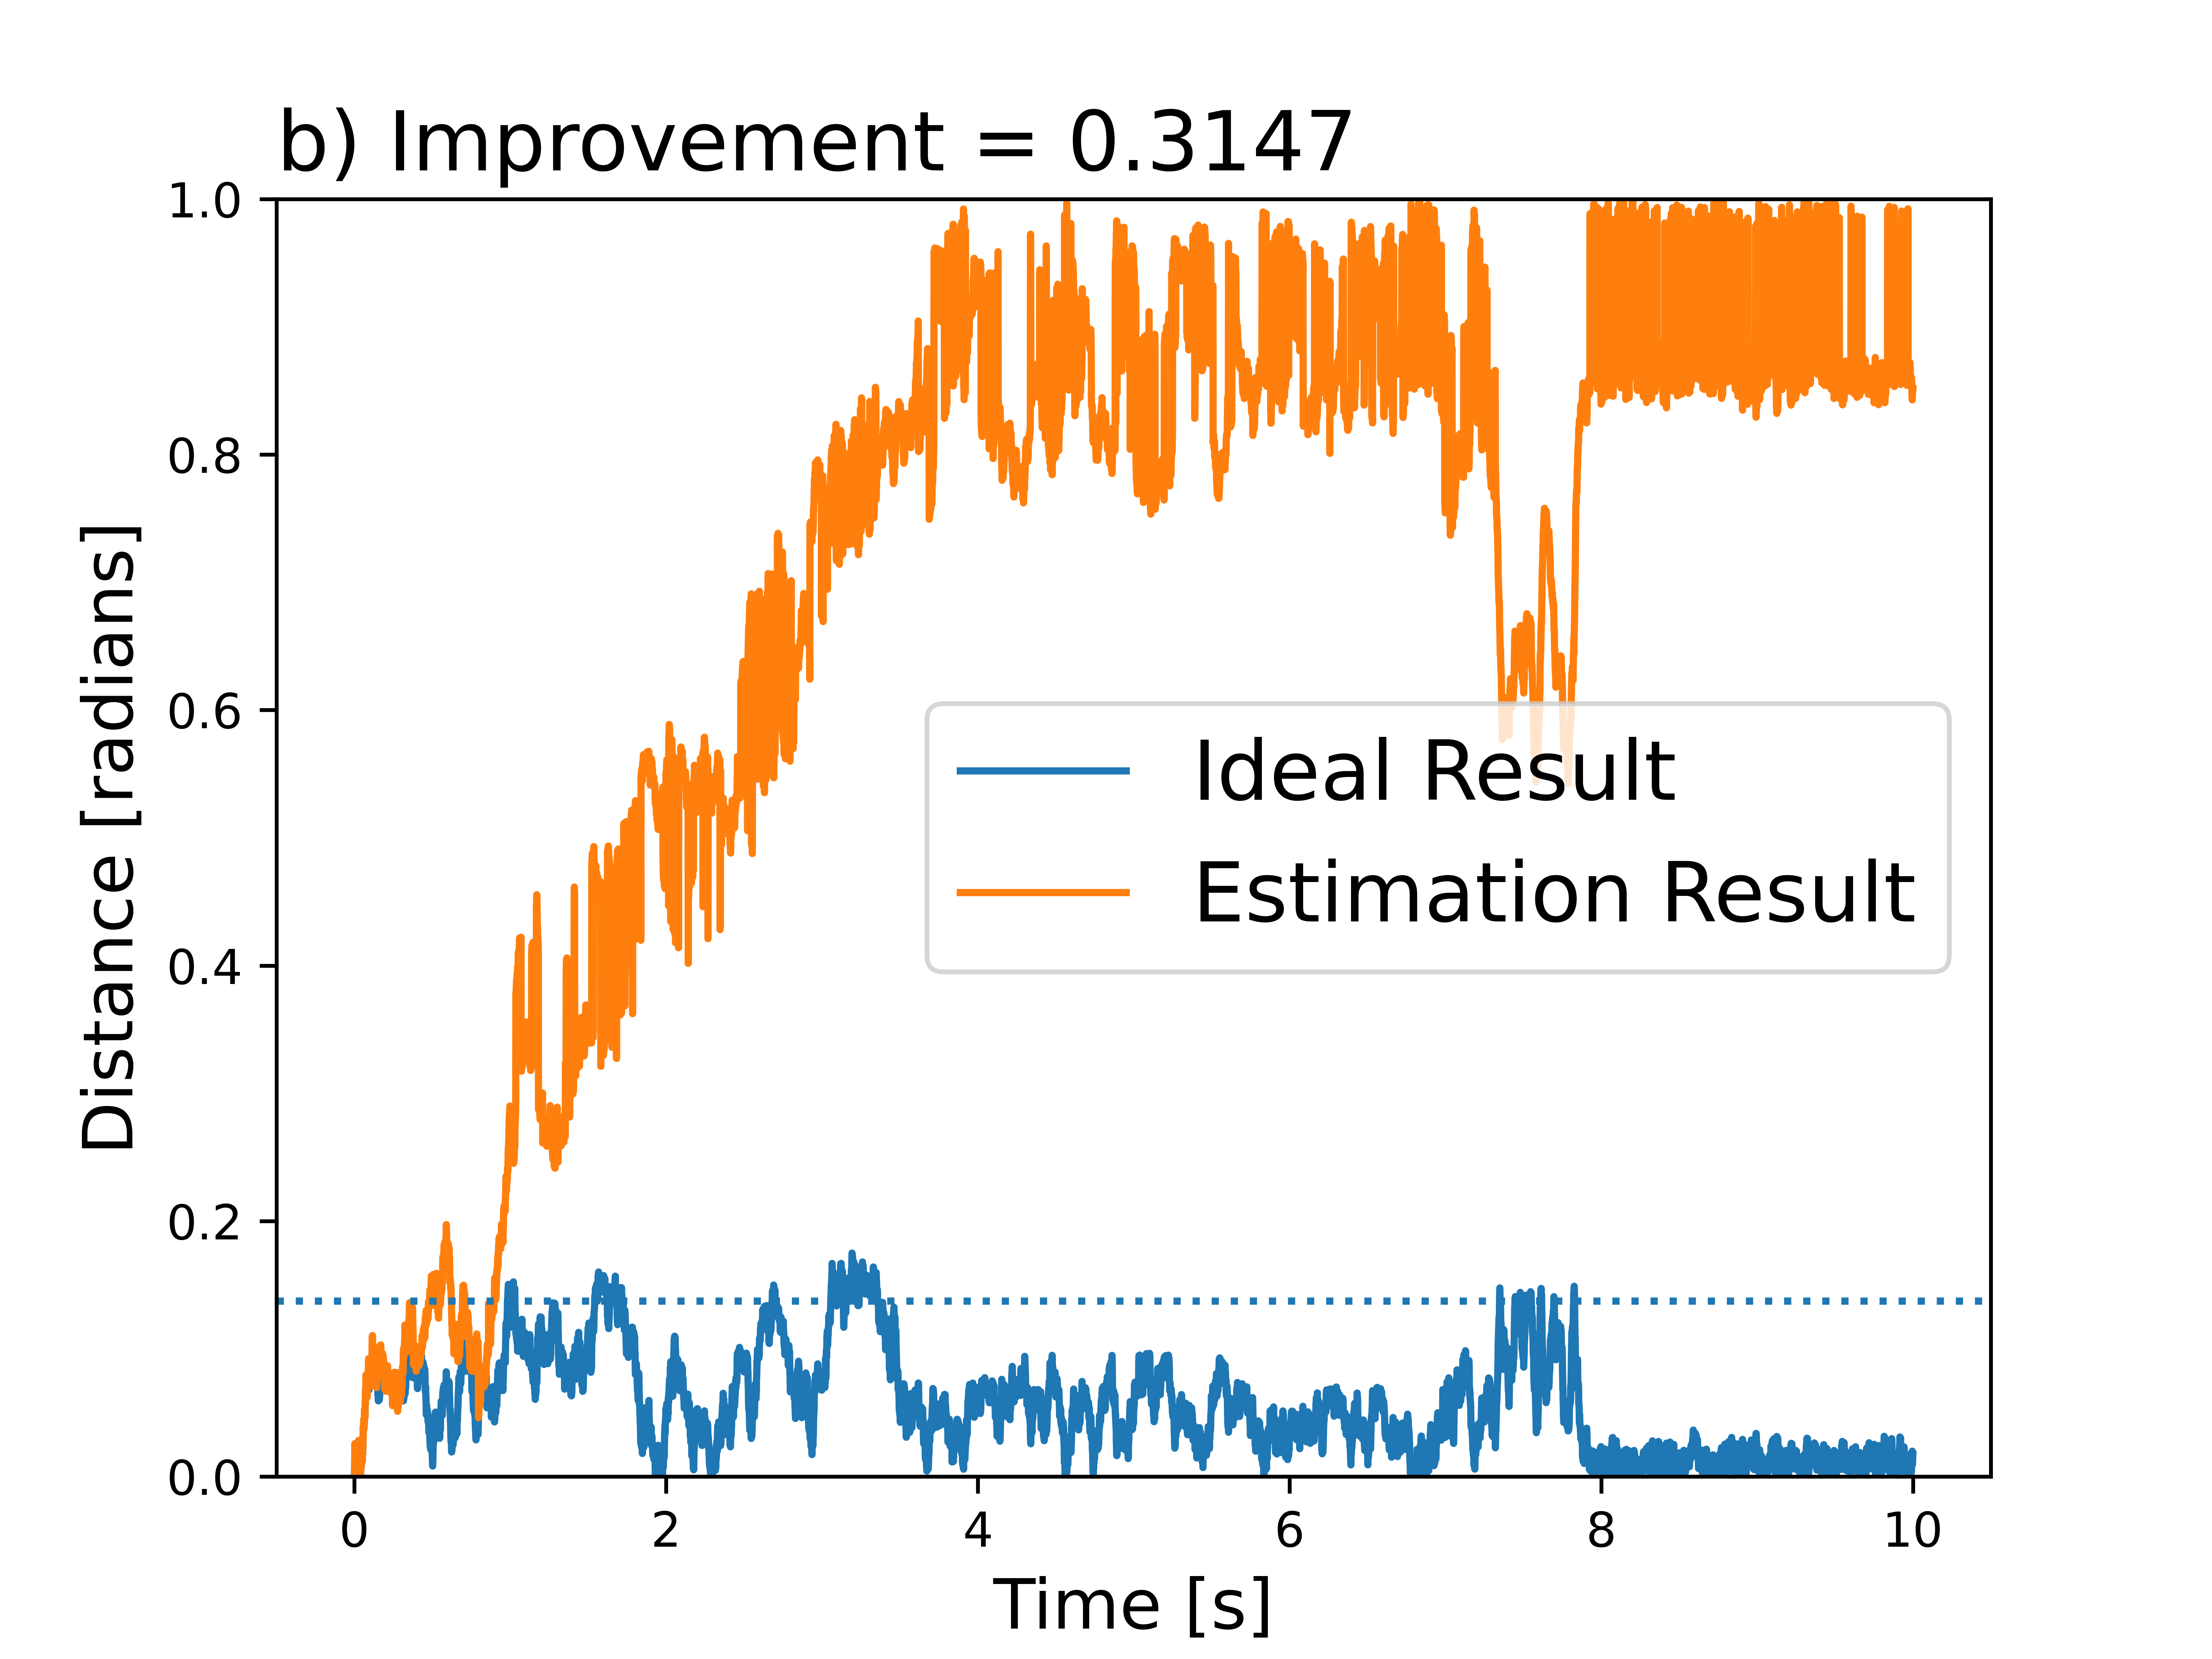
\includegraphics[width=\textwidth]{./Images/beta_6.png}
	\end{subfigure}
	\caption{Model prediction for signal error of $25\%$ when a) $\beta = 5$ and b) $\beta=6$}
\end{figure}

As shown in Figure~\ref{fig:beta}, eventually $\beta$ begins to over
correct our estimate to the extent that we are a full radian away from
the correct result.  The exact value of $\beta$ that will optimise our
performance varies for each choice of angle, therefore we can use it
as variable for finely tuning our results to suit our choice of angles
and our signal error.  In future, we want to also investigate the
possibility of extending our prior $p(\hat{\bf n})$ so we account for not
just the change in orientation after one time step but after 2 or 3
time steps to investigate if we can investigate the auto correlation
of our dimer's motion.

\subsection{Parameter Optimisation Results}
\label{sec:3.3}
We wanted to see if our choice of angles plays a significant role in our model's efficacy. We employed ultranest to analyse the parameter space for our three angles by sampling across the priori of $10^{\circ} \ \& \ 180^{\circ}$. We kept both $\beta$ and $\sigma$ constant during this so we could as these are parameters that can be changed more freely. 

\begin{figure}[h]
	\label{fig:corner}
	\centering
	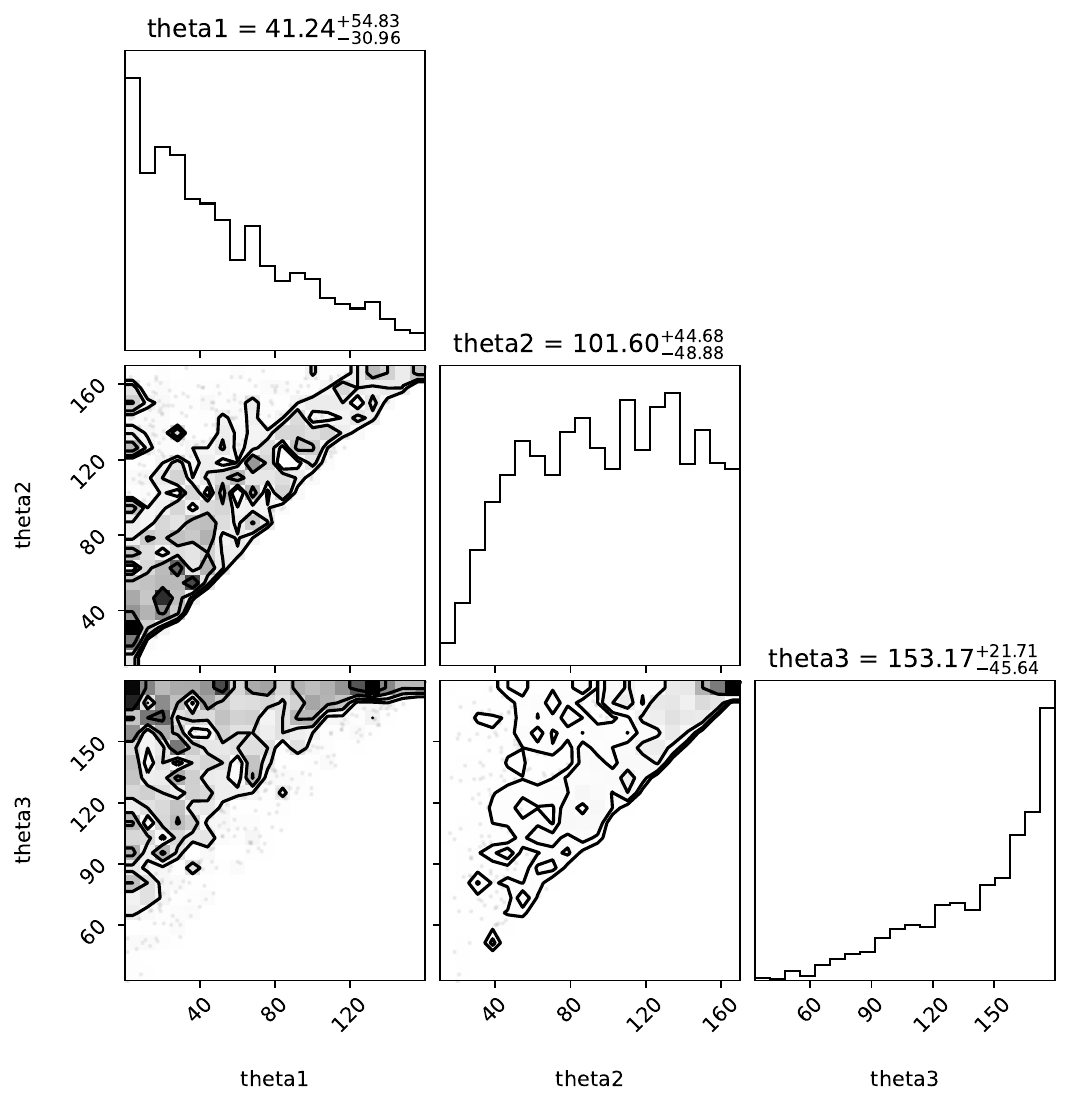
\includegraphics[width=0.45\textwidth]{./Images/corneranglesfreed-1.png}
	\caption{Corner plot mapping combinations of $\theta$ that generate the best improvement}
\end{figure}

Figure~\ref{fig:corner} is the resulting corner plot from our ultranest sampler, darker areas indicate a choice of angles where the model performed better where as lighter areas are where the model did poorer. Overall from the corner plot provided it's clear that there is no direct correlation between our model's performance and the choice of detection angle. While the choice of angles does not provide a direct improvement in our estimation it does determine how finely we can estimate the orientation, for choices of angles that are close together the minimum spacing between our signals is so small that we can't achieve any greater accuracy than dividing the orientation space into 30 reference orientations. We hope to develop our model further in the future by being able to determine the maximum accuracy given that we know the signal error of our measurements.  

As covered in Section~\ref{sec:3.2} our choice for beta can help to improve our estimation by restricting it in the physical space. In addition depending on our choice of angles we are also setting the lower limit for our signal error $\epsilon$, so it may be preferable to choose a selection of angles that allows for a large signal error and then adjust the weighting factor to improve upon our estimation. 


%%%%%%%%%%%%%%%%%%%%%%%%%%%%%%%%%%%%%%%%%%%%%%%%%%%%%%%%%%%%%%%%%%%%%%%%%%%%%%%%
%%%%%%%%%%%%%%%%%%%%%%%%%%%%%%%%%%%%%%%%%%%%%%%%%%%%%%%%%%%%%%%%%%%%%%%%%%%%%%%%
\section{Conclusion}
\label{sec:Conclusion}

We have developed a method for interpreting the dynamics of a trapped
particle based purely on the light scattering pattern. In theory the
model can be applied to any characteristic that impacts the light
scattering pattern produced by the trapped entity. The MSTM package is
flexible in calculating the light scattering for a variety of
micro-particles; so long as there is a distinguishable difference in
the light scattering pattern we can apply this method to characterise
the particle to some degree of accuracy. This has potential to be
applied to characterise particle size and shape that are changing
while in the optical trap. The authors would like to acknowledge and
thank the support for this research from the funding provided by the
Leverhulme Trust.\\



%%%%%%%%%%%%%%%%%%%%%%%%%%%%%%%%%%%%%%%%%%%%%%%%%%%%%%%%%%%%%%%%%%%%%%%%%%%%%%%%
%%%%%%%%%%%%%%%%%%%%%%%%%%%%%%%%%%%%%%%%%%%%%%%%%%%%%%%%%%%%%%%%%%%%%%%%%%%%%%%%
\noindent \textbf{Acknowledgement.} The authors thank the support for this research from the funding provided by the Leverhulme Trust. \\
  
\noindent \textbf{Disclosures.} The authors declare no conflict of interest. \\


%%%%%%%%%%%%%%%%%%%%%%%%%%%%%%%%%%%%%%%%%%%%%%%%%%%%%%%%%%%%%%%%%%%%%%%%%%%%%%%%
%%%%%%%%%%%%%%%%%%%%%%%%%%%%%%%%%%%%%%%%%%%%%%%%%%%%%%%%%%%%%%%%%%%%%%%%%%%%%%%%
\bibliography{bib} 
\bibliographystyle{ieeetr}


\newpage
\appendix
\onecolumn
%%%%%%%%%%%%%%%%%%%%%%%%%%%%%%%%%%%%%%%%%%%%%%%%%%%%%%%%%%%%%%%%%%%%%%%%%%%%%%%%
%%%%%%%%%%%%%%%%%%%%%%%%%%%%%%%%%%%%%%%%%%%%%%%%%%%%%%%%%%%%%%%%%%%%%%%%%%%%%%%%
\section*{Appendix}
\setcounter{table}{0}
\renewcommand{\thetable}{A\arabic{table}}
\label{sec:App1}
\begin{table}[h]
\begin{center}
\caption{\label{tab:A1}
%
Reference Orientations vector components$^*$}
\begin{tabular}{|c|c|c|c|}
\hline\hline
Reference Orientation & $\hat{\bf n}_{i,\ x}$ &  $\hat{\bf n}_{i,\ y}$ &  $\hat{\bf n}_{i,\ z}$ \\
\hline
$1$ & $ 0.29588$ &  $ 0.29588$ & $ 0.90825$ \\
$2$ & $ 0.90825$ &  $ 0.29588$ & $ 0.29588$ \\
$3$ & $ 0.29588$ &  $ 0.90825$ & $ 0.29588$ \\
$4$ & $1.0000$ &  $0.00000$ & $0.00000$ \\
$5$ & $0.00000$ &  $1.0000$ & $0.00000$ \\
$6$ & $0.00000$ &  $0.00000$ & $1.0000$ \\
$7$ & $ 0.29588$ &  $ 0.29588$ & $-0.90825$ \\
$8$ & $ 0.90825$ &  $ 0.29588$ & $-0.29588$ \\
$9$ & $ 0.29588$ &  $ 0.90825$ & $-0.29588$ \\
$10$ & $0.00000$ &  $0.00000$ & $-1.0000$ \\
$11$ & $ 0.29588$ &  $-0.29588$ & $ 0.90825$ \\
$12$ & $ 0.90825$ &  $-0.29588$ & $ 0.29588$ \\
$13$ & $ 0.29588$ &  $-0.90825$ & $ 0.29588$ \\
$14$ & $0.00000$ &  $-1.0000$ & $0.00000$ \\
$15$ & $ 0.29588$ &  $-0.29588$ & $-0.90825$ \\
$16$ & $ 0.90825$ &  $-0.29588$ & $-0.29588$ \\
$17$ & $ 0.29588$ &  $-0.90825$ & $-0.29588$ \\
$18$ & $-0.29588$ &  $ 0.29588$ & $ 0.90825$ \\
$19$ & $-0.90825$ &  $ 0.29588$ & $ 0.29588$ \\
$20$ & $-0.29588$ &  $ 0.90825$ & $ 0.29588$ \\
$21$ & $-1.0000$ &  $0.00000$ & $0.00000$ \\
$22$ & $-0.29588$ &  $ 0.29588$ & $-0.90825$ \\
$23$ & $-0.90825$ &  $ 0.29588$ & $-0.29588$ \\
$24$ & $-0.29588$ &  $ 0.90825$ & $-0.29588$ \\
$25$ & $-0.29588$ &  $-0.29588$ & $ 0.90825$ \\
$26$ & $-0.90825$ &  $-0.29588$ & $ 0.29588$ \\
$27$ & $-0.29588$ &  $-0.90825$ & $ 0.29588$ \\
$28$ & $-0.29588$ &  $-0.29588$ & $-0.90825$ \\
$28$ & $-0.90825$ &  $-0.29588$ & $-0.29588$ \\
$30$ & $-0.29588$ &  $-0.90825$ & $-0.29588$ \\
\hline\hline
\multicolumn{4}{l}{\small *Orientation vector points from centre of sphere 1 to centre of sphere 2.} \\
		\end{tabular}
	\end{center}
\end{table}


\newpage
%%%%%%%%%%%%%%%%%%%%%%%%%%%%%%%%%%%%%%%%%%%%%%%%%%%%%%%%%%%%%%%%%%%%%%%%%%%%%%%%
\begin{table}[h]
  \begin{center}
    \caption{\label{tab:A2}
      % 
      Raw intensities $I_k^*$ and scaled intensities $y_k$}
    \begin{tabular}{|c|c|c|c|c|c|c|}
      \hline\hline
      Reference Orientation  & $I(\hat{\bf n}_i,\ 15^{\circ})$ &  $I(\hat{\bf n}_i, \ 45^{\circ})$ &  $I(\hat{\bf n}_i,\ 90^{\circ})$ & $y(\hat{\bf n}_i, \ 15^{\circ})$ & $y(\hat{\bf n}_i, \ 45^{\circ})$ & $y(\hat{\bf n}_i, \ 90^{\circ})$ \\
\hline
$1$ & $13.371$ & $0.1264$ & $0.0122$ & $-0.5423$ & $-0.4253$ & $-0.4838$ \\
$2$ & $13.237$ & $0.0272$ & $0.0102$ & $0.2429$ & $-1.401$ & $-0.7826$ \\
$3$ & $15.840$ & $0.1072$ & $0.0234$ & $1.337$ &$-0.6142$&	$1.162$ \\
$4$ & $12.657$ & $0.2246$ & $0.0244$ & $-0.0012$ &	$0.5399$ & $0.9695$ \\
$5$ & $15.351$ & $0.0527$ & $0.0221$ & $1.132$ &	$-1.150$ & $1.303$ \\
$6$ & $12.046$ & $0.0916$ & $0.0142$ & $-0.2584$ &	$-0.7676$ &	$-0.1886$ \\
$7$ & $11.376$ & $0.0036$ & $0.0095$ & $-0.5403$ &$-1.633$ & $-0.8792$ \\
$8$ & $13.130$ & $0.2346$ & $0.0095$ & $0.1977$ & $0.6379$ & $-0.8794$ \\
$9$ & $15.975$ & $0.2893$ & $0.0273$ & $1.38724$ & $1.175$ & $1.726$ \\
$10$ & $10.073$ & $0.2933$ & $0.0221$ & $-1.088$	& $1.215$ & $0.9641$ \\
$11$ & $11.371$ & $0.1264$ & $0.0122$ & $-0.5423$ & $-0.4253$ & $-0.4838$ \\
$12$ & $13.238$ & $0.0272$ & $0.0102$ & $0.2429$ &	$-1.401$ & $-0.7826$ \\
$13$ & $15.840$ & $0.1072$ & $0.0234$ & $1.337$ &	$-0.6142$ & $1.162$ \\
$14$ & $15.351$ & $0.0527$ & $0.0244$ & $1.132$ & $-1.150$ & $1.303$ \\
$15$ & $13.376$ & $0.0036$ & $0.0095$ & $-0.5403$ & $-1.633$ & $-0.8792$ \\
$16$ & $13.130$ & $0.2346$ & $0.0095$ & $0.1977$ & $0.6379$ & $-0.8794$ \\
$17$ & $15.957$ & $0.2893$ & $0.0273$ & $1.387$	& $1.175$	& $1.726$ \\
$18$ & $14.199$ & $0.0935$ & $0.0076$ & $0.6472$ & $-0.7496$ & $-1.158$ \\
$19$ & $8.5164$ & $0.3133$ & $0.0076$ & $-1.743$ & $1.411$ & $-1.157$ \\
$20$ & $12.961$ & $0.2420$ & $0.0188$ & $0.1267$ & $0.7113$ & $0.4765$ \\
$21$ & $8.2160$ & $0.3217$ & $0.0142$ & $-1.869$ & $1.495$ & $-0.1890$ \\
$22$ & $14.212$ & $0.2537$ & $0.0102$ & $0.6529$ & $0.8265$ & $-0.7835$ \\
$23$ & $8.9280$ & $0.1398$ & $0.0123$ & $-1.570$ &	$-0.2934$ & $-0.4840$ \\
$24$ & $13.328$ & $0.1964$ & $0.0234$ & $0.2807$ & $0.2624$ & $1.162$ \\
$25$ & $14.199$ & $0.0935$ & $0.0076$ & $0.6472$ & $-0.7496$ & $-1.1580$ \\
$26$ & $8.5164$ & $0.3133$ & $0.0076$ & $-1.743$	& $1.411$ & $-1.157$ \\
$27$ & $12.961$ & $0.2420$ & $0.0188$ & $0.1267$	& $0.7113$ & $0.4765$ \\
$28$ & $14.212$ & $0.2537$ & $0.0102$ & $0.6529$ & $0.8265$ & $-0.7835$ \\
$29$ & $8.9280$ & $0.1398$ & $0.0122$ & $-1.570$ &	$-0.2934$ & $-0.4840$ \\
$30$ & $13.328$ & $0.1964$ & $0.0234$ & $0.2807$ & $0.2624$ & $1.162$ \\
\hline\hline
\multicolumn{7}{l}{\small *$I_k$ values are calculated using MSTM package.}
\end{tabular}
\end{center}
\end{table}


%%%%%%%%%%%%%%%%%%%%%%%%%%%%%%%%%%%%%%%%%%%%%%%%%%%%%%%%%%%%%%%%%%%%%%%%%%%%%%%%
%%%%%%%%%%%%%%%%%%%%%%%%%%%%%%%%%%%%%%%%%%%%%%%%%%%%%%%%%%%%%%%%%%%%%%%%%%%%%%%%
%%%%%%%%%%%%%%%%%%%%%%%%%%%%%%%%%%%%%%%%%%%%%%%%%%%%%%%%%%%%%%%%%%%%%%%%%%%%%%%%
\end{document}
\endinput
